\documentclass[11pt]{article}

\usepackage[T1]{fontenc}
\usepackage{amsmath}
\usepackage{amssymb}
\usepackage{amsthm}
\usepackage{mathrsfs}
\usepackage{booktabs}
\usepackage{microtype}
\usepackage{graphicx}
\usepackage[margin=1in]{geometry}

\newtheorem{theorem}{Theorem}[section]
\newtheorem{lemma}[theorem]{Lemma}
\newtheorem{proposition}[theorem]{Proposition}
\newtheorem{corollary}[theorem]{Corollary}
\newtheorem{definition}[theorem]{Definition}
\newtheorem{remark}[theorem]{Remark}
\newtheorem{example}[theorem]{Example}
\newtheorem{problem}[theorem]{Problem}

\newcommand{\Assign}{\operatorname{Assign}}
\newcommand{\Opt}{\operatorname{Opt}}
\newcommand{\PM}{\operatorname{PM}}
\newcommand{\nnc}{\operatorname{nnc}}
\newcommand{\mnnc}{\operatorname{mnnc}}

\title{Polynomial-Size Signed Tropical Circuits\\for the Assignment Problem}
\author{Shuhuan Wang\\{\small\texttt{ukiyo7@gmail.com}}}
\date{}

\begin{document}
\maketitle

\begin{abstract}
We construct, for every $n$ and every fixed bipartite support with a perfect
matching, a circuit over $\max$, $+$, $-$ and the constant $0$ that outputs the
exact minimum weight of a perfect matching, together with an optimal dual pair,
at every real weight vector.  The circuit has $O(n^{8})$ gates in the dense case
and $O(n^{6}|E|+n^{2}|E|^{2})$ in general, is generated in polynomial time from
the support alone, and assumes no bit width, no separation margin, and no
absence of ties.  This answers a question posed for the assignment problem in
the tropical circuit model, where the corresponding circuits over $\min$ and $+$
alone are exponentially large.

Two mechanisms carry the construction, and neither works without the other.
The first is general: we show that a Boolean observable with a circuit of size
$s$ compiles into a signed tropical circuit of size $O(ms+m^{2}+m\log^{2}m)$ for
its integral over the threshold filtration of the input, the discrete
observation entering only weighted by the gap it would be discontinuous across.
The second is specific: a static schedule of rank stages, together with strict
growth of an alternating reachable set, makes a fixed number of such integrals
suffice, independently of the input.  Neither the smallest positive slack nor
any comparison bit is ever read.

Against this, a circuit that may multiply by arbitrary positive reals but may
not subtract still needs $2^{\Omega(n)}$ addition gates for the same function.
For the assignment value function, positive scalar multiplication does not
remove the exponential barrier, whereas subtraction suffices.  The barrier is
also not an artifact of demanding exactness at unbounded weights.  At weights
drawn from $\{0,1,2\}$ it persists for circuits over $\min$ and $+$ that are
correct only within an additive $\varepsilon<1/2$, and for circuits with
positive scalars that are exact on those weights, and it persists on general
graphs as well as on bipartite ones.
\end{abstract}

\section{Introduction and main results}
\label{sec:intro}

Most classical dynamic programs over a weighted ground set use only the
operations that appear in the definition of the problem they solve.  Circuits
over $\min$ and $+$ formalize that restriction, and lower bounds for them are
lower bounds on that entire algorithmic style~\cite{jukna23-tropical}.  The
restriction is severe.  Jerrum and Snir~\cite{jerrum-snir82} showed that the
assignment value function needs $2^{\Omega(n)}$ gates in this model, and the
Hungarian method~\cite{kuhn55} escapes the bound only by branching on
comparisons, which no such circuit can do.

Two relaxations of the gate set have been studied.  Hertrich and
Stargalla~\cite{hertrich-stargalla26} add multiplication by arbitrary positive
reals and show that the assignment barrier survives: every such circuit for the
support function of the Birkhoff polytope still needs $2^{\Omega(n)}$ addition
gates.  Adding subtraction instead is a different matter.  Hertrich and
Sering~\cite{hertrich-sering25} add it and obtain circuits of size $O(n^{3})$
for the minimum spanning tree value and $O(m^{2}n^{2})$ for maximum flow, and
then ask whether the same is possible for the weight of a minimum weight perfect
matching in a bipartite graph.  Jukna~\cite[Section 6.5, Problem
3]{jukna23-tropical} poses the question in the form it takes for the Hungarian
method: can the branching be replaced by a polynomial-size circuit that is
allowed to subtract.  Hertrich and Stargalla record both questions as open.

We answer them.

\paragraph{The construction.}
Let $H=(L,R,E)$ be a bipartite graph with $|L|=|R|=n$ that has a perfect
matching, and write
\begin{equation}
  \Opt_H(w)=\min_{M\in\PM(H)}\ \sum_{e\in M}w_e,
  \qquad w\in\mathbb R^{E}.
  \label{eq:opt}
\end{equation}
For $H=K_{n,n}$ we write $\Assign_n$ and index the weights by a matrix
$W\in\mathbb R^{n\times n}$.

\begin{theorem}[Main construction]
\label{thm:main}
For every $n\ge1$ there is a circuit $C_n$ whose gates are real input
coordinates, the constant $0$, and binary $\max$, $+$ and $-$, such that
\begin{equation}
  \boxed{\;
  |C_n|=O(n^{8}),
  \qquad
  C_n(W)=\Assign_n(W)
  \quad\text{for every } W\in\mathbb R^{n\times n}.
  \;}
  \label{eq:main}
\end{equation}
The family is uniform: $C_n$ is produced from $n$ by a polynomial-time
generator, and every wire, gate and output index depends on $n$ alone.  The
identity in \eqref{eq:main} holds at ties, at arbitrarily small nonzero
differences, at negative entries and at unbounded entries.  No bit width, no
separation margin and no genericity hypothesis is used.
\end{theorem}

The same generator works for a fixed sparse support, where the size drops.

\begin{theorem}[Fixed support]
\label{thm:main-support}
Given a bipartite $H$ with a perfect matching, a polynomial-time generator
produces a circuit over $\max,+,-,0$ of size
\begin{equation}
  O\bigl(n^{6}|E|+n^{2}|E|^{2}\bigr)
  \label{eq:main-support}
\end{equation}
that outputs, for every $w\in\mathbb R^{E}$, vectors $p\in\mathbb R^{L}$,
$q\in\mathbb R^{R}$, $D\in\mathbb R^{E}$ and a scalar $z$ with
\begin{equation}
  D_{ij}=w_{ij}-p_i-q_j\ \ge\ 0,
  \qquad
  z=\sum_ip_i+\sum_jq_j,
  \label{eq:dual}
\end{equation}
such that the edges with $D_{ij}=0$ contain a perfect matching.  Consequently
$z=\Opt_H(w)$.
\end{theorem}

The output of Theorem~\ref{thm:main-support} is a certificate and not only a
number.  For any perfect matching $N$,
$\sum_{ij\in N}w_{ij}=\sum_ip_i+\sum_jq_j+\sum_{ij\in N}D_{ij}\ge z$, with
equality for a matching inside the zero set, so optimality is checked by a
reader who does not trust the generator.

\paragraph{The mechanism.}
The Hungarian method branches on which slacks are currently zero, and a circuit
has no branch and no comparison bit; Section~\ref{sec:model} makes the
obstruction precise.  Our construction replaces that method by a recurrence
whose only discrete objects are canonical covers of threshold graphs, and it
makes those objects legal in two separate steps.

First, a discrete observation of the slack vector $D$ enters the circuit only
through the integral
$\mathcal C_F(D)=\int_0^{\infty}F(\{e:D_e\le t\})\,dt$ of a Boolean observable
$F$ over the threshold filtration of $D$.  Such an integral is automatically
nonexpansive, $|\mathcal C_F(D)-\mathcal C_F(D')|\le\|D-D'\|_1$, because the
thresholds at which two filtrations differ occupy a set of measure
$\|D-D'\|_1$.  Section~\ref{sec:amplitude} turns that into a compiler:
\emph{a Boolean circuit of size $s$ for $F$ yields a signed tropical circuit of
size $O(ms+m^{2}+m\log^{2}m)$ for $\mathcal C_F$}, by presenting every discrete
bit already multiplied by the gap it would be discontinuous across, so that a
wrong bit is always multiplied by zero.  The integral is the Lov\'asz extension
of $F$ read on complements~\cite{lovasz83}; the size bound is what is new.

Second, continuity alone does not bound the number of updates.  We fix a static
schedule of rank stages $r=0,1,\ldots,n-1$ and prove that, while the rank of the
zero-slack graph equals $r$, one update either raises that rank or strictly
enlarges the canonical alternating reachable set on the left.  The reachable set
starts with at least $n-r$ elements and cannot exceed $n$, so $r+1$ updates at
stage $r$ suffice and the total is $n(n+1)/2$, with no reference to the smallest
positive slack.


\paragraph{The separation.}
The gate sets we compare do not form a chain.  Multiplication by a positive real
is not available to a circuit over $\max,+,-,0$, whose linear pieces all have
integer slopes, and subtraction is not available to a circuit with positive
scalars.  Each extension contains the pure model and neither contains the other,
as in Figure~\ref{fig:diamond}.

\begin{figure}[t]
  \centering
  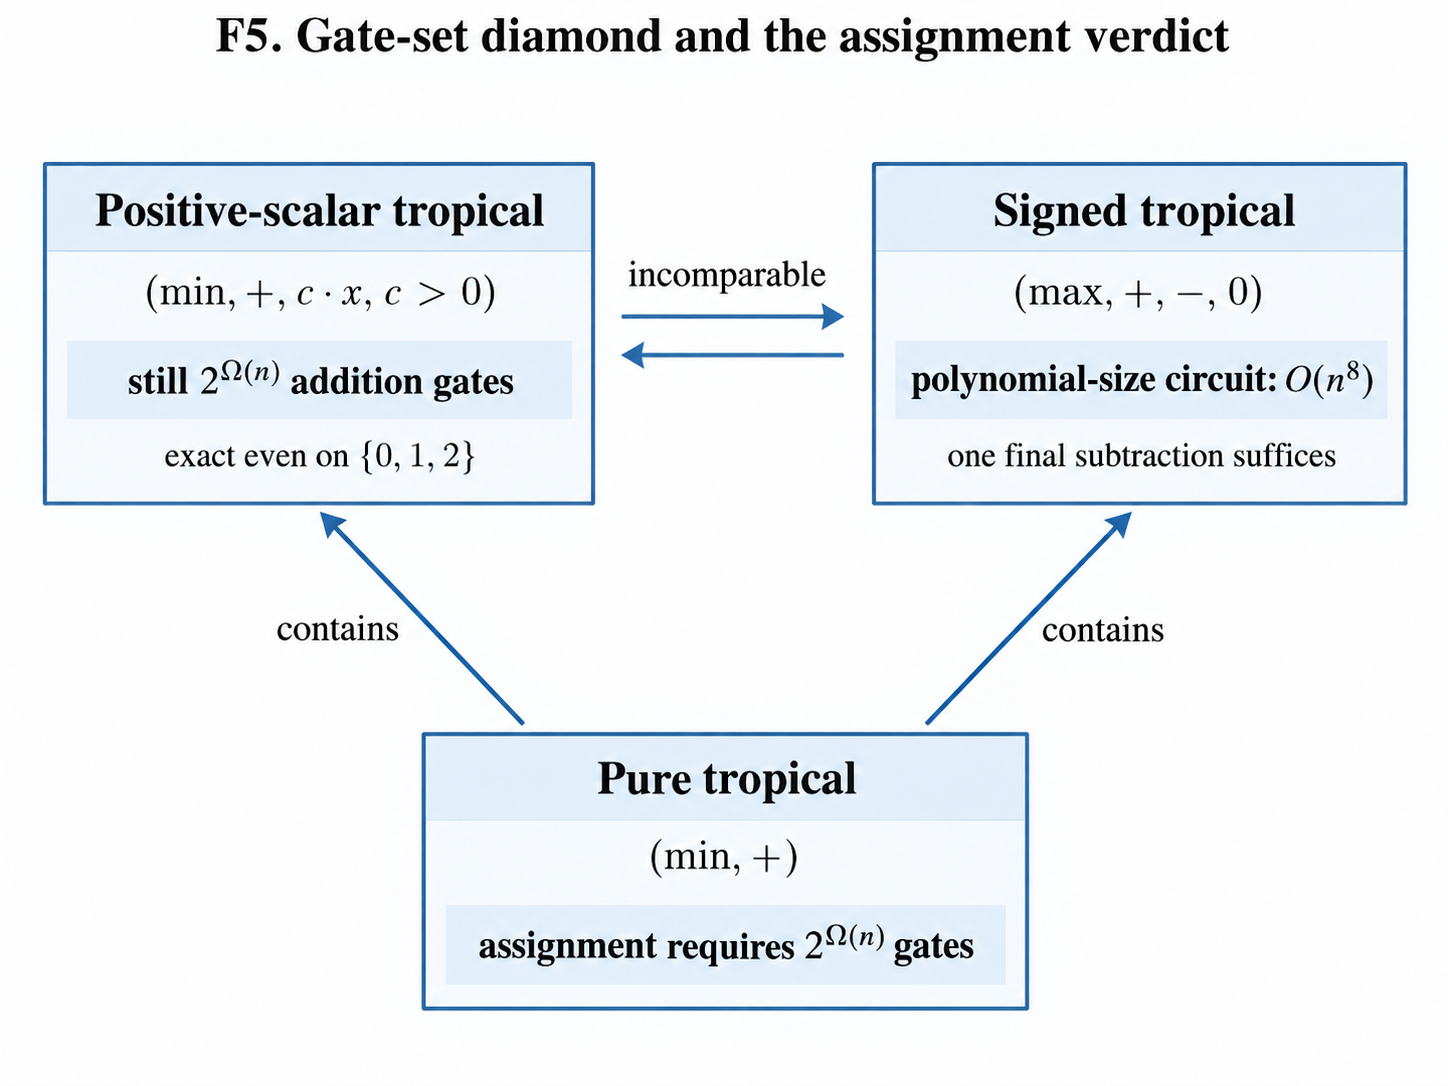
\includegraphics[width=0.86\textwidth]{fig/5.png}
  \caption{The three gate sets of Definition~\ref{def:models} and their verdicts
  on the assignment value function.  The pure model sits below both extensions.
  Neither extension contains the other: a positive-scalar circuit computes
  $\sqrt2\,x$ with one gate, while every function computed over $\max,+,-$ and
  $0$ is piecewise linear with integer slopes.  The two horizontal arrows record
  that incomparability and are not inclusions.}
  \label{fig:diamond}
\end{figure}

For the assignment value function, positive scalar multiplication does not
remove the exponential barrier, whereas subtraction suffices, and
Theorem~\ref{thm:main} uses no scalar other than $\pm1$.  The comparison is
stated for one function rather than as a classification of models.

\begin{theorem}[Separation, with attribution]
\label{thm:separation}
For $\Assign_n$ on $K_{n,n}$:
\begin{enumerate}
  \item every pure tropical circuit correct at all real weights has
        $2^{\Omega(n)}$ gates~\cite{jerrum-snir82};
  \item every positive-scalar tropical circuit correct at all real weights has
        $2^{\Omega(n)}$ addition gates~\cite{hertrich-stargalla26}, a statement
        quoted for the maximum-weight form and transported to \eqref{eq:opt} in
        Section~\ref{sec:separation};
  \item a circuit over $\max,+,-,0$ of size $O(n^{8})$ is exact at all real
        weights, by Theorem~\ref{thm:main}.
\end{enumerate}
\end{theorem}

Parts (1) and (2) are quoted.  What we add on the lower side is robustness.

\begin{theorem}[Bounded-cost robustness]
\label{thm:robust}
Let $n\ge2$, let $\mathsf T=\{0,1,2\}$, let $\mathcal G_+$ denote the set of
addition gates of a circuit, and let $H$ be either $K_{n,n}$ or $K_{2n}$.  In
both models a circuit may use arbitrary finite real constant leaves.
\begin{enumerate}
  \item If a pure tropical circuit $\mathcal G$ satisfies
        $|\mathcal G(w)-\Opt_H(w)|\le\varepsilon$ for every $w\in\mathsf T^{E(H)}$
        with $\varepsilon<1/2$, then
        $|\mathcal G_+|\ge\tfrac12\binom{n}{\lceil n/3\rceil}$.
  \item If a positive-scalar tropical circuit $\mathcal G$ satisfies
        $\mathcal G(w)=\Opt_H(w)$ for every $w\in\mathsf T^{E(H)}$, then
        $|\mathcal G_+|\ge\tfrac12\binom{n}{\lceil n/3\rceil}$.
\end{enumerate}
\end{theorem}

Both bounds are $2^{\Omega(n)}$ and both follow the same route, from five probes
to canonical parses, from those to a fixed vertex scope for every gate, and from
a balanced scope to a product count.  The two parts are separate because the
hypotheses are not interchangeable: the tolerant one uses integrality of
exponents, which a positive scalar gate destroys.  Bipartiteness is never used,
which is why the same constant appears for $K_{2n}$.

\paragraph{A compiler, and three questions it closes.}
The first mechanism is not specific to matchings and is stated on its own in
Section~\ref{sec:amplitude}.  For an observable $F$ on subsets of a ground set
of size $m$ with $F(E)=0$, the threshold integral
$\mathcal C_F(D)=\int_0^{\infty}F(\{e:D_e\le t\})\,dt$ is the Lov\'asz extension
of $F$ read on complements, and a Boolean circuit of size $s$ for $F$ compiles
into a signed tropical circuit of size $O(ms+m^{2}+m\log^{2}m)$ for
$\mathcal C_F$.  When $F$ is monotone the sign-free fragment matches Boolean
complexity exactly: the least size of a circuit over $\min$ and $\max$ computing
$\mathcal C_F$ equals the least size of a monotone Boolean circuit computing $F$,
and likewise for depth.

Jukna, Seiwert and Sergeev~\cite{jukna-seiwert-sergeev20} pose three consecutive
questions that these results answer, and Corollary~\ref{cor:jss} collects them.
Their tropical permanent is $\Assign_n$, so Theorem~\ref{thm:main} answers the
first.  For the second, they reduce a $(\min,+,\max)$ circuit to a monotone
Boolean circuit for bipartite perfect matching, which by
Razborov~\cite{razborov85} and now Cavalar, G\"o\"os, Riazanov, Sofronova and
Sokolov~\cite{cgrss26} needs $2^{n^{1/3-o(1)}}$ gates, against $O(n^{8})$ here.
For the third, they ask whether subtraction helps for bottleneck problems; the
widest perfect matching $\Lambda_n=\max_M\min_{e\in M}x_e$ needs
$2^{n^{1/3-o(1)}}$ gates over $\min$ and $\max$ and has a signed circuit of size
$O(n^{6})$.  The same function separates depth, at $\Omega(n)$ against
$\operatorname{polylog}(n)$.

\paragraph{Related work.}
Lower bounds for circuits over $\min$ and $+$ descend from the monotone
arithmetic circuit bounds of Jerrum and Snir~\cite{jerrum-snir82}; the model and
its state are surveyed by Jukna~\cite{jukna15-tropical, jukna23-tropical}, Jukna
and Seiwert~\cite{jukna-seiwert20} bound what pure dynamic programming can
approximate by a multiplicative factor over all nonnegative weights, and Kluk
and Nederlof~\cite{kluk-nederlof26} bound it for connectivity problems on graphs
of bounded path-width.  We bound it under an additive error on the fixed cost set
$\{0,1,2\}$, which is the form the barrier takes once the weights are bounded.

Enlarging the gate set is the line this paper joins, and it is short.  Hertrich
and Sering~\cite{hertrich-sering25} add subtraction and obtain polynomial-size
circuits for the minimum spanning tree value and for maximum flow.  Hertrich,
Kober and Loho~\cite{hertrich-kober-loho26} obtain them for weighted basis
maximization over regular matroids, by building a $(+,\times,\div)$ circuit of
size $O(n^{3})$ for the basis generating polynomial and tropicalizing it, so that
division becomes subtraction.  Fomin, Grigoriev and Koshevoy~\cite{fgk16} give
subtraction-free circuits of polynomial size for the generating polynomials of
spanning trees and of directed spanning trees; tropicalized, they give
polynomial-size circuits over $(\min,+,-)$ for minimum-cost arborescences,
against the exponential lower bound of Jerrum and Snir~\cite{jerrum-snir82} over
$(\min,+)$.  Hertrich and
Stargalla~\cite{hertrich-stargalla26} add positive scalars instead and keep the
exponential bound for the Birkhoff support function.  Hertrich and
Loho~\cite{hertrich-loho26} bound circuit size below by the extension complexity
of the underlying polytope for monotone and input-convex circuits, and identify
subtraction as what blocks the same bound in general.  We add subtraction and
obtain polynomial-size circuits for the assignment value function, and we show
that the positive-scalar barrier survives on a finite cost set.  Two differences
are worth naming.  The tropicalization route is unavailable here, because the
generating polynomial of the bipartite perfect matchings is the permanent; the
subtractions in Section~\ref{sec:circuit} come from potential updates rather than
from divisions.  Their placement is also what carries the construction, since
Jukna, Seiwert and Sergeev~\cite{jukna-seiwert-sergeev20} show that admitting
$-w_e$ alongside each input $w_e$ shortens a $(\min,+)$ circuit by at most a
quadratic factor.

Lower bounds that route a computation through a decomposition of the instance are
the ambient technique: branch decompositions and their tangle duality are due to
Robertson and Seymour~\cite{robertson-seymour91}, bucket
elimination~\cite{dechter-bucket} is the dynamic programming template, and width
lower bounds of this shape appear in Bova et al.~\cite{bova16-kc}, Mengel and
Wallon~\cite{mengel-wallon20} and Korhonen~\cite{korhonen21-mwis}.
Appendix~\ref{app:lower} follows that shape, with the vertex scope of a gate in
place of a decomposition node and a count of perfect matchings in place of a
rectangle count.  On the algorithmic side the Hungarian method~\cite{kuhn55}
solves the bipartite case by branching on which slacks are currently zero, and
Edmonds~\cite{edmonds65} solves the general case with odd-set duals whose support
depends on the input; Section~\ref{sec:frontier} explains why the second
obstruction is the one that survives here.
\paragraph{Organization.}
Section~\ref{sec:model} fixes the model and explains why polynomial-time
solvability gives no circuit of this kind.  Section~\ref{sec:amplitude} proves the
compiler, which is independent of matchings.  Section~\ref{sec:circuit} contains
the recurrence, its progress proof, its termination, and what the circuit can
and cannot select.  Section~\ref{sec:separation}
proves Theorem~\ref{thm:robust} and places it against the quoted bounds.
Section~\ref{sec:verification} separates the kinds of evidence behind the
implementation.  Section~\ref{sec:frontier} states where bipartiteness is used
and what remains.

\section{Model and construction overview}
\label{sec:model}

\begin{definition}[Gate sets]
\label{def:models}
All circuits are finite directed acyclic graphs with unrestricted fan-out whose
sources are the real input coordinates and the constant $0$.  Size is the number
of gates, and every gate is counted.
\begin{itemize}
  \item A \emph{pure tropical} circuit has binary $\min$ and $+$ gates.
  \item A \emph{positive-scalar tropical} circuit adds the unary gates
        $x\mapsto cx$ for $c\in\mathbb R_{>0}$.
  \item A \emph{signed tropical} circuit has binary $\max$, $+$ and $-$ gates.
\end{itemize}
The three models share the same sources.  A pure circuit is therefore a
positive-scalar circuit outright, and rewriting every $\min$ gate as
$\min(x,y)=x-\max(x-y,0)$ turns it into a signed circuit of at most three times
the size, which is the containment drawn in Figure~\ref{fig:diamond}.  The lower
bounds of Section~\ref{sec:separation} are proved in the two larger models that
also admit arbitrary finite real constant leaves.
\end{definition}

A signed tropical circuit has no multiplication, no division, no rounding, no
comparison gate returning a discontinuous bit, no data-dependent indirect
addressing and no optimization oracle.  The abbreviation
$\min(x,y)=x-\max(x-y,0)$ costs three gates and is counted as such.  Every
function computed is continuous and piecewise linear with integer slopes, which
is why the gate sets of Definition~\ref{def:models} form the diamond of
Figure~\ref{fig:diamond} and not a chain.

The support $H$ is part of the circuit description.  It is not a real-valued
runtime input, and its edges carry a fixed enumeration.  Feasibility of $H$ is
decided once, at generation time, by an unweighted matching computation.

\paragraph{Why polynomial time is not enough.}
The Hungarian method maintains a slack matrix $D\ge0$ and repeatedly selects the
smallest slack crossing the current cover.  Both the selection and the cover
depend on which entries are currently zero, and that dependence is
discontinuous: an arbitrarily small perturbation of $w$ can change the cover and
hence the next update direction.  A circuit over $\max,+,-,0$ computes a
continuous function, so it cannot read such a decision.  Nor can it be obtained
by simulating a finite-precision implementation, since the theorem is required
to hold at all real weights, including ties and arbitrarily small gaps.

\paragraph{Notation.}
The following symbols are fixed throughout.

\begin{center}
\begin{tabular}{@{}ll@{}}
\toprule
Symbol & Meaning \\
\midrule
$H=(L,R,E)$, $n$, $m$ & bipartite support, $|L|=|R|=n$, $m=|E|$ \\
$\PM(H)$, $\chi_M$ & perfect matchings of $H$, indicator of $M$ \\
$\Opt_H(w)$, $\Assign_n$ & value \eqref{eq:opt}; the case $H=K_{n,n}$ \\
$\mathsf T$ & the cost set $\{0,1,2\}$ \\
$p,q,D,z$ & potentials, slack $D_{ij}=w_{ij}-p_i-q_j$, value $\sum p+\sum q$ \\
$G^{0}(D)$, $G_t(D)$, $G_k$ & zero-slack graph; $\{e:D_e\le t\}$; $G_{s_k}$ \\
$s_0\le\cdots\le s_m$, $\Delta_k$ & sorted slacks with $s_0=0$; gaps $s_{k+1}-s_k$ \\
$\nu(G)$, $S(G)$, $T(G)$ & matching number; canonical reachable pair \\
$\tau,\lambda_i,\mu_j$ & bottleneck levels \eqref{eq:bottleneck} \\
$U_r$, $a_i$, $c_j$ & stage-$r$ update \eqref{eq:update} and its potentials \\
$\mathcal C_F$ & threshold integral \eqref{eq:threshold-integral} \\
$\Lambda_n$ & widest perfect matching, Corollary~\ref{cor:bottleneck} \\
$\kappa_P$, $\alpha_P$, $V_h$ & parse constant, parse exponent, vertex scope \\
$s(H)$ & splitting number, Definition~\ref{def:splitting} \\
$\nnc$, $\mnnc$ & maxout network complexity, general and monotone \\
$\operatorname{Lat}$, $\operatorname{Mon}$, $\operatorname{STrop}$, $\operatorname{Bool}$ & least size over $\{\min,\max\}$, $\{\wedge,\vee\}$, $\{\max,+,-,0\}$, Boolean \\
\bottomrule
\end{tabular}
\end{center}

\paragraph{Two-line summary of the construction.}
Normalize $D_e=w_e-\min_fw_f$ and set $p_i=\min_fw_f$, $q_j=0$, so
\eqref{eq:dual} holds with $D\ge0$.  Then apply the fixed schedule
\begin{equation}
  U_0^{1},\ U_1^{2},\ U_2^{3},\ \ldots,\ U_{n-1}^{n},
  \label{eq:schedule}
\end{equation}
where $U_r$ is the update of Section~\ref{sec:circuit} and the exponents denote
repeated composition, not a data-dependent loop.  Each $U_r$ moves potential from
rows to columns by an amount read off from the threshold graphs of $D$, keeps
$D\ge0$, and preserves \eqref{eq:dual}.  After the schedule the zero set of $D$
contains a perfect matching, and $z$ is the optimum.

\section{Compiling Boolean observers on a threshold filtration}
\label{sec:amplitude}

This section is independent of matchings.  Fix a finite ground set $E$ with
$m=|E|$ and a vector $D\in\mathbb R_{\ge0}^{E}$.

\begin{definition}[Threshold filtration and threshold integral]
\label{def:filtration}
The \emph{threshold filtration} of $D$ is the family
$G_t(D)=\{e\in E: D_e\le t\}$ for $t\ge0$.  For a Boolean observable
$F\colon2^{E}\to\{0,1\}$ with $F(E)=0$, the \emph{threshold integral} of $F$ at
$D$ is
\begin{equation}
  \mathcal C_F(D)=\int_0^{\infty}F\bigl(G_t(D)\bigr)\,dt .
  \label{eq:threshold-integral}
\end{equation}
\end{definition}

Sorting the entries of $D$ and prepending a zero gives
\begin{equation}
  0=s_0\le s_1\le\cdots\le s_m,
  \qquad
  \Delta_k=s_{k+1}-s_k,
  \qquad
  G_k=G_{s_k}(D),
  \label{eq:sorted}
\end{equation}
for $0\le k<m$.  Order statistics are continuous functions of $D$ and are
computed by a sorting network~\cite{batcher68} of $O(m\log^{2}m)$ comparators,
each comparator costing one $\max$ and one $\min$.  The network is fixed in
advance and no element label is carried through it.  Sorting is both legal and
useful here: Jukna and Seiwert~\cite{jukna-seiwert-sorting20} show that access
to the sorted weights can speed up a pure circuit exponentially.

\begin{proposition}[Two readings of the threshold integral]
\label{prop:two-readings}
Let $F\colon2^{E}\to\mathbb R$ satisfy $F(E)=0$, and define $\mathcal C_F$ by
\eqref{eq:threshold-integral}.  For every $D\in\mathbb R_{\ge0}^{E}$,
\begin{equation}
  \mathcal C_F(D)=\sum_{k=0}^{m-1}\Delta_k\,F(G_k),
  \label{eq:gap-sum}
\end{equation}
and, writing $g(S)=F(E\setminus S)$ so that $g(\varnothing)=0$,
\begin{equation}
  \mathcal C_F(D)=\int_0^{\infty}g\bigl(\{e:D_e\ge t\}\bigr)\,dt ,
  \label{eq:lovasz}
\end{equation}
which is the Lov\'asz extension of the set function $g$ evaluated at
$D$~\cite{lovasz83}.
\end{proposition}

\begin{proof}
The set $G_t(D)$ is constant for $t$ in $[s_k,s_{k+1})$, because no entry of $D$
lies strictly between two consecutive sorted values, and it equals $E$ for
$t\ge s_m$, where $F$ vanishes by hypothesis.  Splitting the integral at the
sorted values gives \eqref{eq:gap-sum}.  The sets $\{e:D_e\ge t\}$ and
$E\setminus G_t(D)$ differ only at the finitely many $t$ that are entries of
$D$, a null set, which gives \eqref{eq:lovasz}.
\end{proof}

\begin{figure}[t]
  \centering
  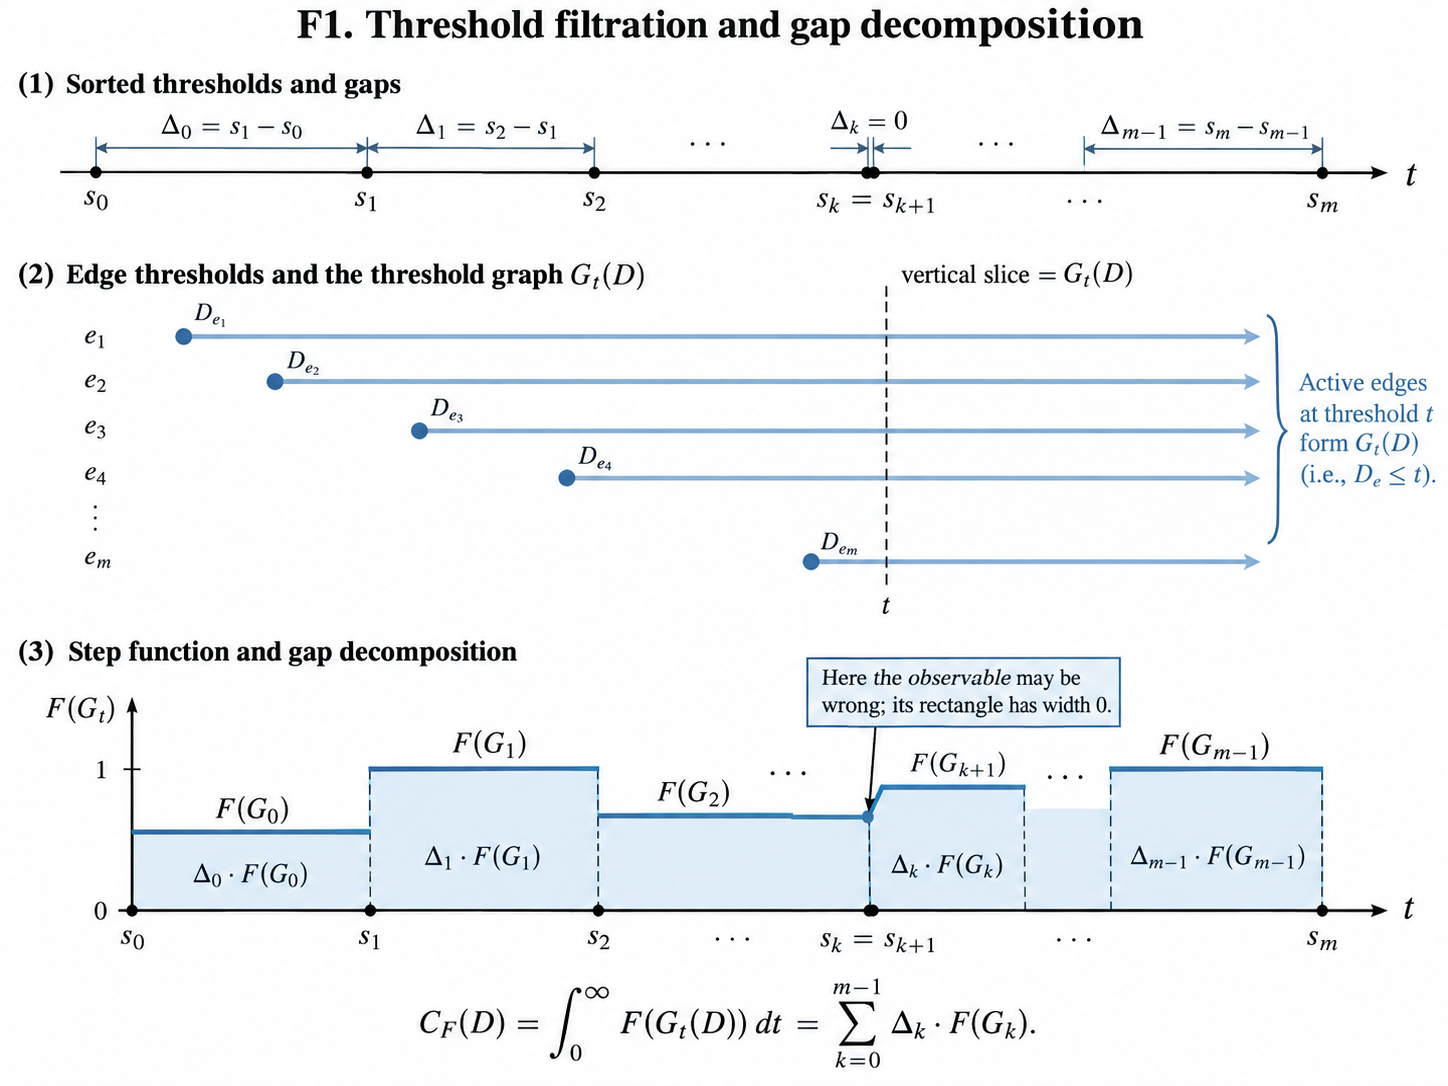
\includegraphics[width=\textwidth]{fig/1.png}
  \caption{The three readings of $\mathcal C_F$.  Panel (1) is the sorted slack
  vector and its gaps.  Panel (2) draws each edge $e$ as a ray starting at
  $t=D_e$, so the vertical slice at $t$ is $G_t(D)$.  Panel (3) is the step
  function $t\mapsto F(G_t)$, whose area is $\mathcal C_F(D)$ and whose
  decomposition into rectangles of width $\Delta_k$ is \eqref{eq:gap-sum}; the
  heights are drawn schematically, and the same decomposition holds for the
  integer-valued observables of Corollary~\ref{cor:integer-observable}.  At the
  marked coincidence $s_k=s_{k+1}$ the observable may report the wrong graph,
  and its rectangle has width $0$, which is Lemma~\ref{lem:lift}.}
  \label{fig:filtration}
\end{figure}

The extension in \eqref{eq:lovasz} is classical and requires no submodularity;
the observables used in Section~\ref{sec:circuit} are not submodular.  What this
section adds is a size bound: a Boolean circuit for $F$ compiles into a signed
tropical circuit for $\mathcal C_F$.

\begin{lemma}[The threshold integral is nonexpansive]
\label{lem:lipschitz}
For all $D,D'\in\mathbb R_{\ge0}^{E}$,
\begin{equation}
  \bigl|\mathcal C_F(D)-\mathcal C_F(D')\bigr|\ \le\ \|D-D'\|_1 .
  \label{eq:lipschitz}
\end{equation}
\end{lemma}

\begin{proof}
If $G_t(D)\ne G_t(D')$ then some $e$ satisfies $D_e\le t<D'_e$ or
$D'_e\le t<D_e$, so $t$ lies in an interval of length $|D_e-D'_e|$.  The set of
such $t$ therefore has measure at most $\|D-D'\|_1$, and the two integrands
differ by at most $1$ there and by $0$ elsewhere.
\end{proof}

Lemma~\ref{lem:lipschitz} settles continuity without any case analysis at ties.
The circuit-level statement below is its discrete counterpart: an observable is
allowed to be wrong exactly where the weight it carries vanishes.

\begin{lemma}[Exact membership at amplitude]
\label{lem:bit}
For every $e\in E$ and every $k<m$,
\begin{equation}
  \Delta_k-\min\bigl(\max(D_{e}-s_k,0),\ \Delta_k\bigr)
  \ =\ \Delta_k\cdot\mathbf1\bigl[\,e\in G_k\,\bigr].
  \label{eq:bit}
\end{equation}
\end{lemma}

\begin{proof}
The value $D_e$ occurs in the sorted list, so either $D_e\le s_k$ or
$D_e\ge s_{k+1}$.  In the first case $\max(D_e-s_k,0)=0$ and the left side is
$\Delta_k$.  In the second case $D_e-s_k\ge\Delta_k$, the inner minimum is
$\Delta_k$, and the left side is $0$.  If $\Delta_k=0$ both cases give $0$.
\end{proof}

\begin{lemma}[Lifting a Boolean circuit]
\label{lem:lift}
Let $F$ be a Boolean circuit with $s$ gates over $\wedge,\vee,\neg$.  There is a
circuit over $\max,+,-$ with $O(s)$ gates which, given the inputs of $F$
presented as values in $\{0,\Delta\}$ for a value $\Delta\ge0$ supplied as a
wire, outputs $\Delta\cdot F(\text{inputs})$.  If $\Delta=0$ every wire of the
lifted circuit carries $0$.
\end{lemma}

\begin{proof}
Represent the Boolean value $b$ by $\Delta b$.  Then
$\Delta(b_1\wedge b_2)=\max(\Delta b_1+\Delta b_2-\Delta,0)$,
$\Delta(b_1\vee b_2)=\max(\Delta b_1,\Delta b_2)$ and
$\Delta(\neg b)=\Delta-\Delta b$, each a constant number of permitted gates and
each returning a value in $\{0,\Delta\}$.  Correctness at $\Delta>0$ follows by
induction on the gates of $F$.  At $\Delta=0$ all three formulas return $0$ from
inputs $0$, so every wire is $0$.
\end{proof}

\begin{theorem}[Compiler]
\label{thm:compiler}
Let $F=(F_1,\ldots,F_N)\colon2^{E}\to\{0,1\}^{N}$ satisfy $F_u(E)=0$ for every
$u$ and be computed by one Boolean circuit of size $s$ over $\wedge,\vee,\neg$
reading the indicator vector of its argument.  Then the vector
$(\mathcal C_{F_1},\ldots,\mathcal C_{F_N})$ is computed at every
$D\in\mathbb R_{\ge0}^{E}$ by a signed tropical circuit of size
\begin{equation}
  O\bigl(ms+mN+m^{2}+m\log^{2}m\bigr).
  \label{eq:compiler-size}
\end{equation}
\end{theorem}

\begin{proof}
Sort $D$ at $O(m\log^{2}m)$ gates, which also supplies every $\Delta_k$ at one
subtraction each.  For each of the $m$ gaps, Lemma~\ref{lem:bit} produces the
$m$ membership values of $G_k$ at amplitude $\Delta_k$ using $O(m)$ gates, and
Lemma~\ref{lem:lift} lifts the whole Boolean circuit once, at $O(s)$ gates,
returning all $N$ values $\Delta_kF_u(G_k)$ together.  At $\Delta_k=0$ every one
of them is $0$ whatever the lifted observer would have computed, which is what
\eqref{eq:gap-sum} requires, since each term is multiplied by $\Delta_k$.
Accumulating $N$ running sums over the $m$ gaps costs $O(mN)$ gates, and
Proposition~\ref{prop:two-readings} identifies the $u$-th sum with
$\mathcal C_{F_u}(D)$.
\end{proof}

Sharing one Boolean circuit across the $N$ outputs is what keeps the cost of a
whole vector of observables at $O(ms)$ rather than $O(Nms)$, and
Section~\ref{sec:circuit} uses it with $N=2n$.

\begin{corollary}[Integer observables, at the cost of their bit length]
\label{cor:integer-observable}
Let $f\colon2^{E}\to\{0,1,\ldots,2^{L}-1\}$ satisfy $f(E)=0$ and let one Boolean
circuit of size $s$ output the $L$ bits of $f$.  Then
$\int_0^{\infty}f(G_t(D))\,dt$ has a signed tropical circuit of size
$O\bigl(ms+mL+m^{2}+m\log^{2}m\bigr)$, and it is Lipschitz in $\|\cdot\|_1$ with
constant $\max_S f(S)$.
\end{corollary}

\begin{proof}
Apply Theorem~\ref{thm:compiler} to the vector of the $L$ output bits, which
returns $\Delta_kb_0,\ldots,\Delta_kb_{L-1}$ at each gap.  Recover the value by
Horner's rule: set $y_L=0$ and $y_j=y_{j+1}+y_{j+1}+\Delta_kb_j$ for
$j=L-1,\ldots,0$, so that $y_0=\Delta_kf(G_k)$ at $O(L)$ gates per gap.  At
$\Delta_k=0$ every lifted bit is $0$ and so is $y_0$.  Accumulate over the gaps
and apply Proposition~\ref{prop:two-readings}.  The Lipschitz bound follows from
\eqref{eq:lipschitz} applied to the Boolean observables $\mathbf1[f\ge j]$ for
$1\le j\le\max_Sf(S)$, which vanish at $E$ and sum to $f$.
\end{proof}

The cost is the bit length of the observable, not its range, so the compiler
applies to counting observables such as $\nu(G)$ and not only to predicates.
A signed-valued observable is handled as a difference of two nonnegative ones.

\subsection{Monotone observables, where the correspondence is exact}
\label{sec:monotone}

For a monotone observable the compiled integral has a closed form and its
complexity in the sign-free fragment is not merely bounded by the Boolean one
but equal to it.  Throughout this subsection circuits have no constant leaves.

\begin{proposition}[Sugeno form]
\label{prop:sugeno}
Let $g\colon2^{E}\to\{0,1\}$ be monotone with $g(\varnothing)=0$, and put
$F(S)=g(E\setminus S)$.  Then for every $D\in\mathbb R_{\ge0}^{E}$,
\begin{equation}
  \mathcal C_F(D)=\max_{A:\,g(A)=1}\ \min_{e\in A}D_e ,
  \label{eq:sugeno}
\end{equation}
with the convention that the maximum over an empty family is $0$.
\end{proposition}

\begin{proof}
By \eqref{eq:lovasz}, $\mathcal C_F(D)=\int_0^{\infty}g(\{e:D_e\ge t\})\,dt$.
The set $\{e:D_e\ge t\}$ shrinks as $t$ grows and $g$ is monotone, so the
integrand is the indicator of an interval $[0,t^{*}]$, where $t^{*}$ is the
largest $t$ admitting some $A$ with $g(A)=1$ and $D_e\ge t$ for all $e\in A$.
That supremum is the right side of \eqref{eq:sugeno}.
\end{proof}

\begin{definition}[Lattice circuits]
\label{def:lattice}
A \emph{lattice circuit} has binary $\min$ and $\max$ gates and no constants.
Write $\operatorname{Lat}(h)$ for the least size of a lattice circuit computing
$h$, and $\operatorname{Mon}(g)$ for the least size of a Boolean circuit over
$\wedge,\vee$ without constants computing $g$; $\operatorname{LatDepth}$ and
$\operatorname{MonDepth}$ denote the corresponding depths.
\end{definition}

\begin{theorem}[Exact equivalence in the monotone case]
\label{thm:lattice}
Let $g$ be monotone with $g(\varnothing)=0$ and $g(E)=1$, and let
$\Lambda_g(D)$ denote the right side of \eqref{eq:sugeno}.  Then
\[
  \operatorname{Lat}(\Lambda_g)=\operatorname{Mon}(g),
  \qquad
  \operatorname{LatDepth}(\Lambda_g)=\operatorname{MonDepth}(g).
\]
\end{theorem}

\begin{proof}
Given a Boolean circuit $C$ for $g$, let $C^{\mathrm{lat}}$ replace every
$\wedge$ by $\min$ and every $\vee$ by $\max$, keeping the graph.  Induction on
the gates gives, for every $t\in\mathbb R$,
\[
  \mathbf1\bigl[C^{\mathrm{lat}}(D)\ge t\bigr]
  =C\bigl(\mathbf1[D_{e_1}\ge t],\ldots,\mathbf1[D_{e_m}\ge t]\bigr),
\]
because $\min(a,b)\ge t$ iff both do and $\max(a,b)\ge t$ iff one does.  Hence
$C^{\mathrm{lat}}(D)$ is the largest $t$ with $g(\{e:D_e\ge t\})=1$, which is
$\Lambda_g(D)$, and the size and depth are unchanged.  Conversely a lattice
circuit for $\Lambda_g$ restricted to $\{0,1\}^{E}$ is a Boolean circuit over
$\wedge,\vee$, and $\Lambda_g(\mathbf1_S)=g(S)$ by monotonicity, so it computes
$g$ at the same size and depth.
\end{proof}

\subsection{Simulating back, and what it costs to prove lower bounds}
\label{sec:reverse}

\begin{theorem}[Polynomial equivalence with Boolean circuit size]
\label{thm:equivalence}
Let $g\colon2^{E}\to\{0,1\}$ with $g(\varnothing)=0$, let $F(S)=g(E\setminus S)$,
and write $\operatorname{STrop}(\mathcal C_F)$ for the least size of a signed
tropical circuit computing $\mathcal C_F$ on $\mathbb R_{\ge0}^{E}$ and
$\operatorname{Bool}(g)$ for the least size of a Boolean circuit computing $g$.
Then
\begin{equation}
  \operatorname{Bool}(g)\ \le\ O\bigl(\operatorname{STrop}(\mathcal C_F)^{2}\bigr),
  \qquad
  \operatorname{STrop}(\mathcal C_F)\ \le\ O\bigl(m\operatorname{Bool}(g)+m^{2}+m\log^{2}m\bigr).
  \label{eq:equivalence}
\end{equation}
\end{theorem}

\begin{proof}
The right inequality is Theorem~\ref{thm:compiler}.  For the left one, let
$\mathcal S$ be a signed tropical circuit of size $S$ for $\mathcal C_F$ and
restrict its inputs to $\{0,1\}^{E}$.  Every leaf then carries an integer of
absolute value at most $1$, and each of $\max$, $+$ and $-$ at most doubles the
largest absolute value present, so every wire carries an integer of absolute
value at most $2^{S}$ and fits in $O(S)$ bits.  Simulating one gate on $O(S)$-bit
integers costs $O(S)$ Boolean gates for $+$ and $-$ and $O(S)$ for $\max$, by
comparison and selection, so the whole circuit is simulated by $O(S^{2})$ Boolean
gates.  Finally $\mathcal C_F(\mathbf1_S)=g(S)$, by \eqref{eq:lovasz} applied to
the vector that is $1$ on $S$ and $0$ elsewhere, so the simulation computes $g$.
\end{proof}

\begin{corollary}[A barrier, on this class]
\label{cor:barrier}
If $\mathcal C_F$ requires signed tropical circuits of size $L(m)$, then $g$
requires Boolean circuits of size $\Omega\bigl((L(m)-O(m^{2}))/m\bigr)$.  A
super-polynomial lower bound for a compiled integral therefore carries a
super-polynomial lower bound for an explicit Boolean function.
\end{corollary}

The barrier comes from the upper bound in \eqref{eq:equivalence}, not from the
simulation, and it applies only to compiled integrals.

\begin{remark}[The compiler does not reach the assignment value function]
\label{rem:not-braid}
A compiled integral is linear on each region where the coordinates of $D$ are in
a fixed order, since by \eqref{eq:gap-sum} the sets $G_k$ are then constant.
The function
\[
  \Assign_2(W)=\min(w_{11}+w_{22},\ w_{12}+w_{21})
\]
is not.  At $W=(0,10,11,12)$ in the coordinate order
$w_{11}<w_{12}<w_{21}<w_{22}$ the first argument is smaller, $12<21$, and at
$W'=(0,1,10,20)$ in the same order the second is, $11<20$.  So one application
of Theorem~\ref{thm:compiler} cannot compute $\Assign_n$ even at $n=2$, and some
operation outside the compiled class is needed.  Section~\ref{sec:circuit}
supplies one.
\end{remark}

The same two points, read as the two alternating paths of a dual-feasible slack
matrix with zero matching $\{L_1R_1,L_2R_2\}$ and positive slacks
$x_1,x_2$ at $L_0$ and $x_3,x_4$ into a free right vertex, show that a shortest
alternating path distance $\min(x_1+x_4,x_2+x_3)$ is not a compiled integral
either.  Bottleneck data lives on the arrangement $D_e=D_f$; path sums live on
the finer arrangement $\sum_{e\in P}D_e=\sum_{e\in Q}D_e$.

\subsection{A bottleneck problem where subtraction helps}
\label{sec:bottleneck}

\begin{corollary}[Widest perfect matching]
\label{cor:bottleneck}
Let $\Lambda_n(x)=\max_{M\in\PM(K_{n,n})}\min_{e\in M}x_e$ for
$x\in\mathbb R_{\ge0}^{E(K_{n,n})}$.  Then
\[
  \operatorname{Lat}(\Lambda_n)=\operatorname{Mon}(\textsc{Match}_n)\ \ge\ 2^{n^{1/3-o(1)}},
  \qquad
  \operatorname{STrop}(\Lambda_n)=O(n^{6}),
\]
where $\textsc{Match}_n\colon\{0,1\}^{n\times n}\to\{0,1\}$ decides whether the
bipartite graph given by its adjacency matrix has a perfect matching.
\end{corollary}

\begin{proof}
Apply Proposition~\ref{prop:sugeno} and Theorem~\ref{thm:lattice} with
$g=\textsc{Match}_n$, which is monotone with $g(\varnothing)=0$ and $g(E)=1$, to
identify $\Lambda_n$ with $\mathcal C_F$ for $F(S)=\textsc{Match}_n(E\setminus S)$
and $\operatorname{Lat}(\Lambda_n)$ with $\operatorname{Mon}(\textsc{Match}_n)$.
The quoted bound is Cavalar, G\"o\"os, Riazanov, Sofronova and
Sokolov~\cite{cgrss26}; Razborov's $n^{\Omega(\log n)}$~\cite{razborov85} already
makes it super-polynomial.  For the upper bound, $F$ is computed by negating the
$m=n^{2}$ input bits and running the circuit of
Proposition~\ref{prop:observer} at $r=n-1$, of size $O(n^{2}m)=O(n^{4})$, and
Theorem~\ref{thm:compiler} with $N=1$ gives $O(ms+m^{2}+m\log^{2}m)=O(n^{6})$.
\end{proof}

\begin{remark}[The same function separates depth]
\label{rem:depth-separation}
Raz and Wigderson~\cite{raz-wigderson92} prove that monotone circuits for
bipartite perfect matching require depth $\Omega(n)$, so
$\operatorname{LatDepth}(\Lambda_n)=\Omega(n)$ by Theorem~\ref{thm:lattice}.
Bipartite matching was recently placed in deterministic
$\mathsf{NC}$~\cite{cgnc26}, which supplies a Boolean circuit of polynomial size
and polylogarithmic depth for $\textsc{Match}_n$; the compiler runs its $m$ gaps
in parallel, sorts in depth $O(\log^{2}m)$ and sums in a balanced tree, so
$\Lambda_n$ has a signed tropical circuit of polynomial size and depth
$\operatorname{polylog}(n)$.  Neither statement uses the schedule of
Section~\ref{sec:circuit}.
\end{remark}

Nothing above mentions the assignment problem.  Section~\ref{sec:circuit}
supplies the observables for which the compiled integrals must be composed
rather than used once, and the schedule that bounds how many are needed.

\begin{remark}[The observables used below]
\label{rem:observers}
For a bipartite graph $G$ on $L\cup R$ with $|L|=|R|=n$, write $\nu(G)$ for the
size of a maximum matching, $S(G)\subseteq L$ for the set of left vertices
reachable by alternating paths from the unmatched ones, and $T(G)=N_G(S(G))$.
The observables compiled in Section~\ref{sec:circuit} are
\begin{equation}
  F^{L}_{r,i}(G)=\mathbf1[\nu(G)\le r]\,\mathbf1[i\in S(G)],
  \qquad
  F^{R}_{r,j}(G)=\mathbf1[\nu(G)\le r]\,\mathbf1[j\in T(G)],
  \label{eq:observables}
\end{equation}
for $r<n$.  Both vanish at $G=E$, where $\nu=n>r$, so
Definition~\ref{def:filtration} applies.  Both are polynomial-time functions of
the $m$ adjacency bits with $(n,E)$ fixed, hence have explicit Boolean circuits;
Proposition~\ref{prop:observer} gives one of size $O(n^{2}m)$.
\end{remark}

\section{A rank-staged assignment circuit}
\label{sec:circuit}

Throughout this section $D\in\mathbb R_{\ge0}^{E}$, and $G^{0}(D)$ denotes the
graph of entries equal to zero.  For a matching $M$ of a bipartite graph $G$, a
vertex is free if no edge of $M$ meets it, and an alternating path from a free
left vertex alternates between edges outside and inside $M$.  Write $S(G)$ for
the set of left vertices reachable by such paths and $T(G)=N_G(S(G))$.  Both are
independent of the maximum matching chosen, and
\begin{equation}
  |S(G)|-|T(G)|=n-\nu(G),
  \qquad
  N_G(S(G))=T(G),
  \label{eq:cover}
\end{equation}
so $(L\setminus S(G))\cup T(G)$ is a minimum vertex cover.  Every vertex of
$T(G)$ is matched by every maximum matching, and its partner lies in $S(G)$.
These facts are classical; Lemma~\ref{lem:canonical} states them in the form
used below and proves them.

\subsection{The update}

Fix an integer $r\in\{0,\ldots,n-1\}$, part of the static schedule
\eqref{eq:schedule}.  Let $F^{L}_{r,i}$ and $F^{R}_{r,j}$ be the observables
\eqref{eq:observables} of Remark~\ref{rem:observers}, put
\begin{equation}
  a_i=\mathcal C_{F^{L}_{r,i}}(D),
  \qquad
  c_j=\mathcal C_{F^{R}_{r,j}}(D),
  \label{eq:ac}
\end{equation}
and define the simultaneous update
\begin{equation}
  (U_rD)_{ij}=D_{ij}-a_i+c_j .
  \label{eq:update}
\end{equation}
Every $a_i$ and $c_j$ is a threshold integral of the old $D$, so
Theorem~\ref{thm:compiler} realizes all $2n$ of them, and
Lemma~\ref{lem:lipschitz} makes each of them nonexpansive in $D$.  Written out
through \eqref{eq:gap-sum} they are the gap sums
$a_i=\sum_k\Delta_kF^{L}_{r,i}(G_k)$ and $c_j=\sum_k\Delta_kF^{R}_{r,j}(G_k)$;
the circuit never forms a factor $F^{L}_{r,i}(G_k)$ on its own.

\begin{lemma}[Feasibility]
\label{lem:feasible}
$U_rD\ge0$ for every $D\ge0$ and every $r<n$.
\end{lemma}

\begin{proof}
Fix $ij\in E$ and put $d=D_{ij}$.  For $t\ge d$ the edge $ij$ lies in $G_t(D)$,
and $N_{G_t}(S(G_t))=T(G_t)$ gives
$F^{L}_{r,i}(G_t)\le F^{R}_{r,j}(G_t)$, so the integrand of $a_i-c_j$ is at most
$0$ there.  For $t<d$ it is at most $1$.  Hence
$a_i-c_j\le\int_0^{d}1\,dt=d$.
\end{proof}

\begin{proposition}[What the update is]
\label{prop:bottleneck}
Assume $\nu(G^{0}(D))=r$ and set
\begin{equation}
  \tau=\min_{|M|=r+1}\ \max_{e\in M}D_e,
  \qquad
  \lambda_i=\min_{\substack{|M|=r\\ i\notin V(M)}}\ \max_{e\in M}D_e,
  \qquad
  \mu_j=\min_{i:\,ij\in E}\ \max(\lambda_i,D_{ij}),
  \label{eq:bottleneck}
\end{equation}
the minima being over matchings of $H$, with $\max\varnothing=0$ and with
$\lambda_i=+\infty$ when $H$ has no $r$-matching avoiding $i$, in which case
$(\tau-\lambda_i)_+=0$.  The value $\tau$ is finite because $H$ has a perfect
matching and $r<n$.  Then
\begin{equation}
  a_i=(\tau-\lambda_i)_+,
  \qquad
  c_j=(\tau-\mu_j)_+,
  \qquad
  (U_rD)_{ij}=D_{ij}-(\tau-\lambda_i)_++(\tau-\mu_j)_+ .
  \label{eq:bottleneck-update}
\end{equation}
\end{proposition}

\begin{proof}
\emph{Step 1.}  The quantity $\tau$ is the least $t$ with $\nu(G_t(D))>r$, so
the guard $\mathbf1[\nu(G_t)\le r]$ is on exactly for $t<\tau$, and
$\nu(G_t)=r$ there.

\emph{Step 2.}  For $t<\tau$, Lemma~\ref{lem:canonical}(4) gives
$i\in S(G_t)\iff\nu(G_t-i)=r$, and $\lambda_i$ is the least $t$ at which
$G_t$ carries a matching of size $r$ avoiding $i$.  Since $\nu(G_t-i)$ is
nondecreasing in $t$ and capped at $\nu(G_t)=r$, the set
$\{t<\tau: i\in S(G_t)\}$ is the interval $[\lambda_i,\tau)$, of length
$(\tau-\lambda_i)_+$.

\emph{Step 3.}  For $t<\tau$, $j\in T(G_t)$ holds iff some $i$ has $ij\in G_t$
and $i\in S(G_t)$, that is $\max(\lambda_i,D_{ij})\le t$.  The least such $t$ is
$\mu_j$, and the same interval argument gives $c_j=(\tau-\mu_j)_+$.
\end{proof}

\begin{figure}[t]
  \centering
  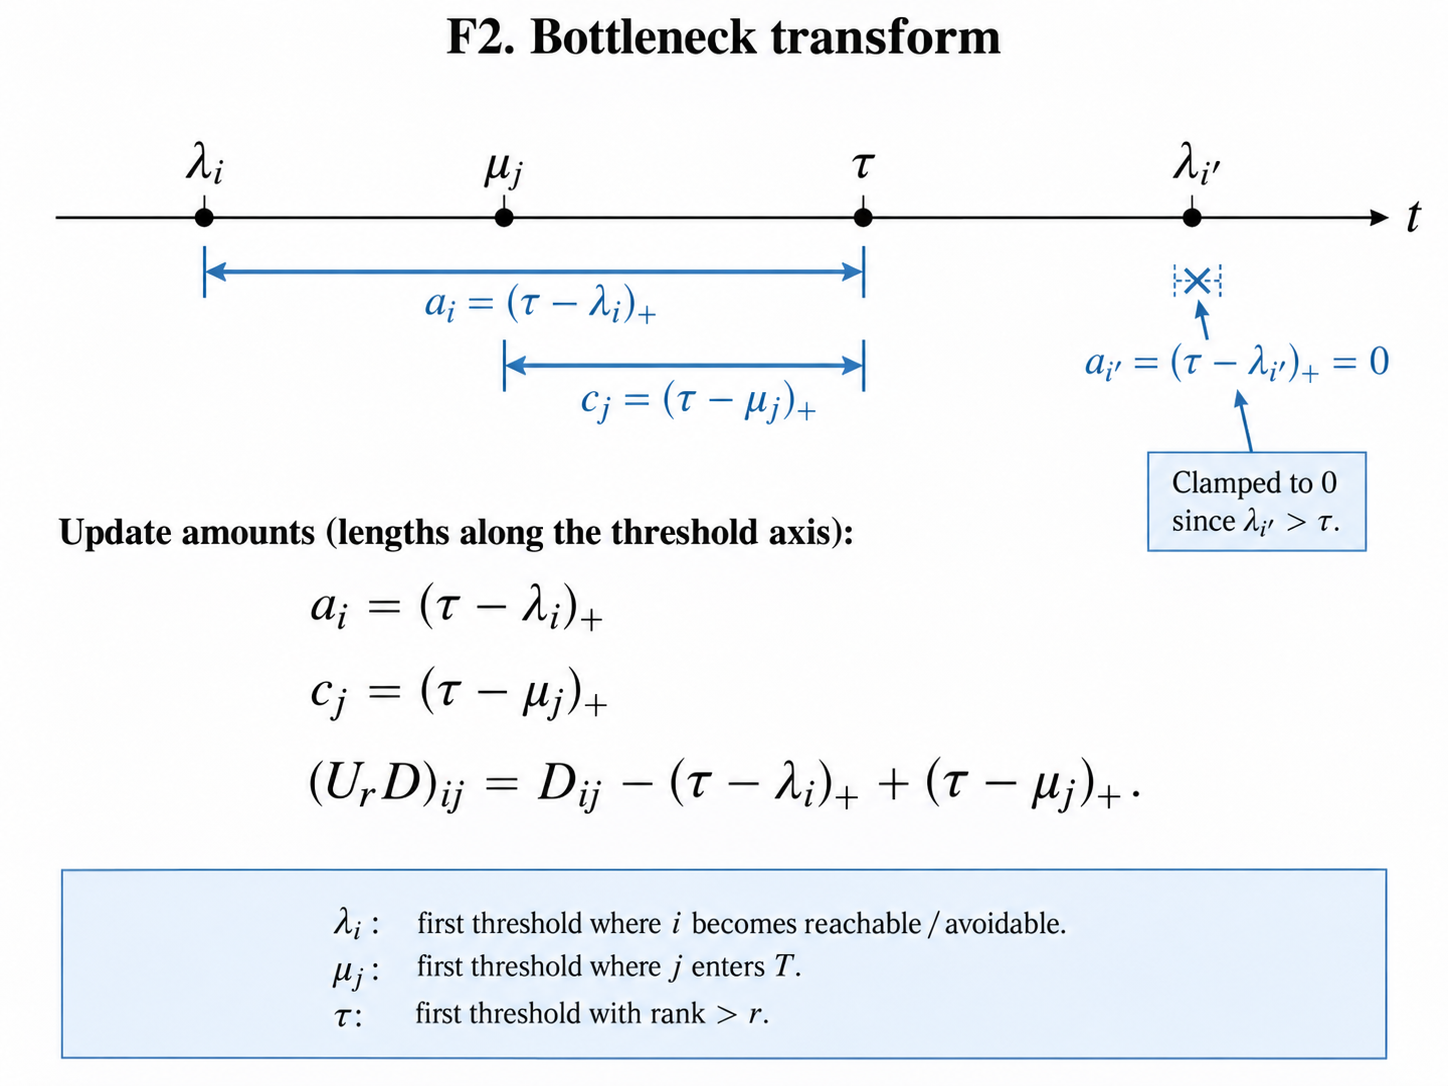
\includegraphics[width=0.82\textwidth]{fig/2.png}
  \caption{Proposition~\ref{prop:bottleneck} as lengths on the threshold axis.
  Each left vertex enters the reachable set at $\lambda_i$ and each right vertex
  at $\mu_j$; the guard switches off at $\tau$.  The potentials are the lengths
  of the overlaps, and a vertex whose threshold lies beyond $\tau$ receives
  nothing.}
  \label{fig:bottleneck}
\end{figure}

So $U_r$ is a bottleneck distance transform of the filtration, and the sorted
values, the graphs $G_k$ and the sets $S(G_k)$, $T(G_k)$ are a representation of
it rather than part of it.  Feasibility can be read off \eqref{eq:bottleneck}
directly: the choice of $i$ in $\mu_j$ gives $\mu_j\le\max(\lambda_i,D_{ij})$,
and if $\lambda_i\ge D_{ij}$ then $\mu_j\le\lambda_i$ and
$(U_rD)_{ij}\ge D_{ij}$, while if $\lambda_i<D_{ij}$ then $\mu_j\le D_{ij}$ and
$(U_rD)_{ij}\ge\min(\tau,\lambda_i)\ge0$ when $\tau>D_{ij}$ and
$\ge D_{ij}-\tau\ge0$ otherwise.

\begin{lemma}[Objective shift]
\label{lem:shift}
$\Opt_H(D)=\sum_ia_i-\sum_jc_j+\Opt_H(U_rD)$.
\end{lemma}

\begin{proof}
A perfect matching meets every row and every column once, so the cost of each
individual matching changes by the constant $\sum_ia_i-\sum_jc_j$.
\end{proof}

\begin{lemma}[Inactive stages]
\label{lem:inactive}
If $\nu(G^{0}(D))>r$ then $a=c=0$ and $U_rD=D$.
\end{lemma}

\begin{proof}
Every $G_t(D)$ contains $G^{0}(D)$, so $\nu(G_t)>r$ and the guard in
\eqref{eq:observables} vanishes at every $t$.
\end{proof}

\subsection{Strict progress at an active stage}

\begin{theorem}[Progress dichotomy]
\label{thm:progress}
Assume $\nu(G^{0}(D))=r<n$ and write $S_0=S(G^{0}(D))$, $T_0=T(G^{0}(D))$.  Then
\begin{equation}
  \boxed{\;
  \nu\bigl(G^{0}(U_rD)\bigr)>r
  \qquad\text{or}\qquad
  \Bigl(\nu\bigl(G^{0}(U_rD)\bigr)=r
  \ \text{ and }\
  S\bigl(G^{0}(U_rD)\bigr)\supsetneq S_0\Bigr).
  \;}
  \label{eq:dichotomy}
\end{equation}
\end{theorem}

\begin{figure}[t]
  \centering
  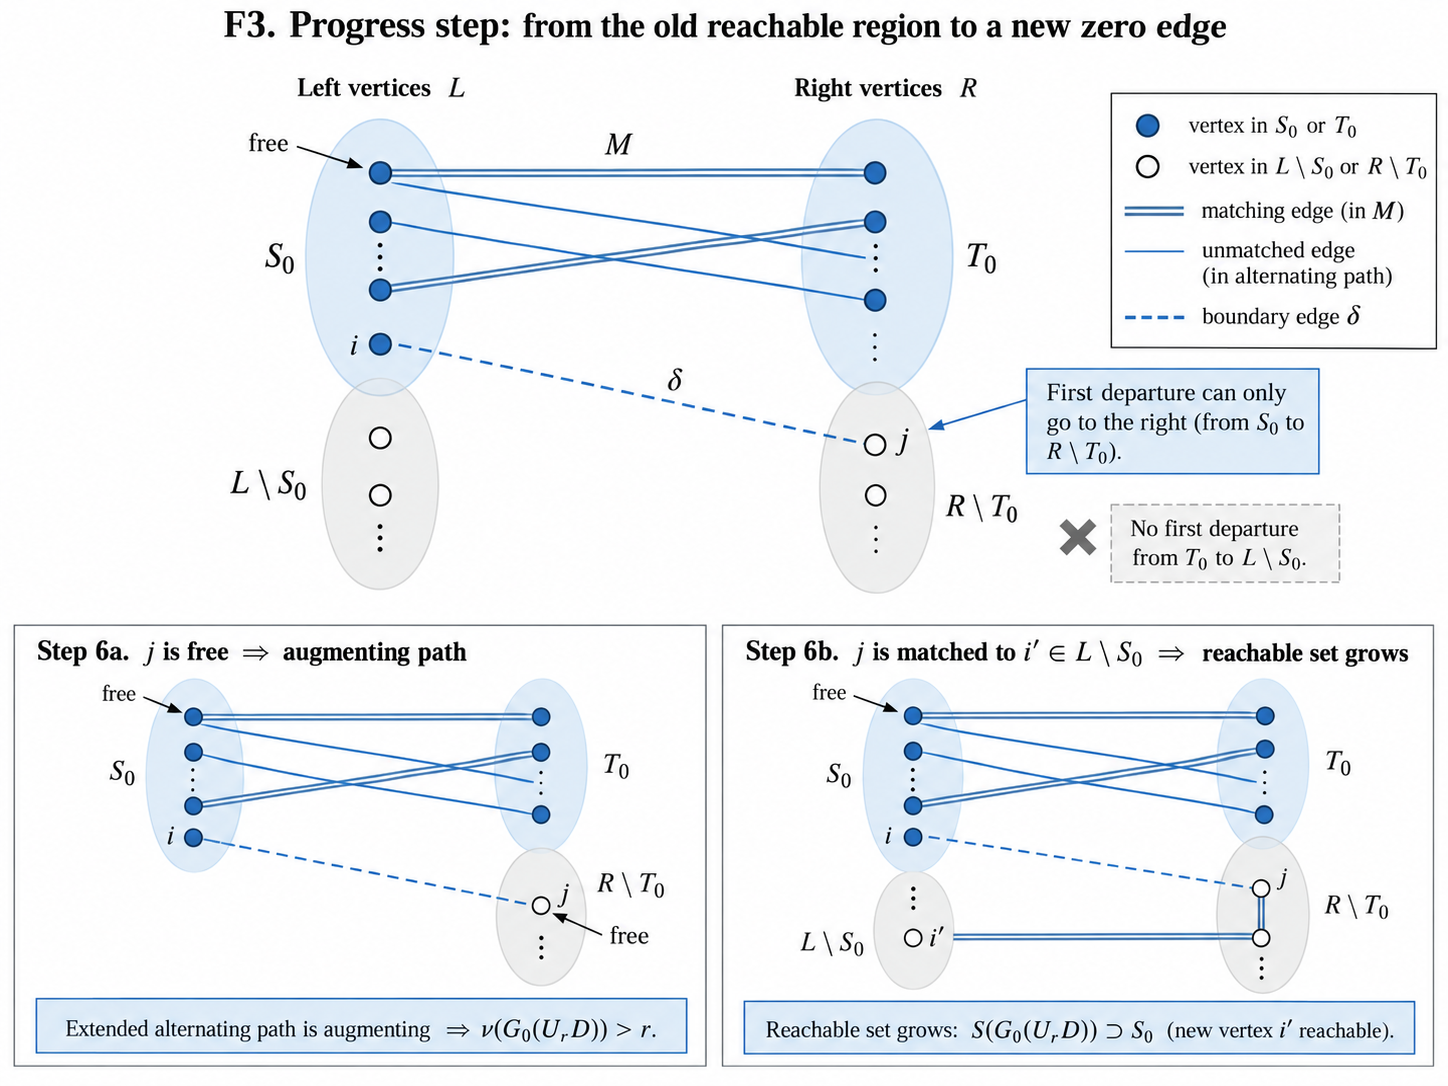
\includegraphics[width=\textwidth]{fig/3.png}
  \caption{The situation in Steps 3 to 6 of Theorem~\ref{thm:progress}.  The
  top panel shows the old reachable pair $(S_0,T_0)$, the matching $M$ inside
  it, and the boundary edge $ij$ of slack $\delta$; Step 4 rules out a first
  departure from $T_0$ to $L\setminus S_0$, so the only way out is to the right.
  The lower panels are the two branches of Step 6.  The figure writes
  $G_0$ for the zero-slack graph $G^{0}$ of the text.}
  \label{fig:progress}
\end{figure}

\begin{proof}
Fix a maximum matching $M$ of $G^{0}(D)$, so $|M|=r$, and set
\[
  \tau=\min\bigl\{\,s_k:\ 0\le k\le m,\ \nu(\{D\le s_k\})>r\,\bigr\},
  \qquad
  \text{$k$ \emph{active}} :\iff s_k<\tau .
\]
The set is nonempty because $\{D\le s_m\}=E$ and $\nu(H)=n>r$, and $\tau>0$
because $\{D\le s_0\}=G^{0}(D)$ has rank $r$.  Since $\tau$ is one of the sorted
values, the active widths telescope to $\sum_{k\ \mathrm{active}}\Delta_k=\tau$.

\emph{Step 0: what holds below $\tau$.}  For $k$ active,
\begin{align*}
  G^{0}(D)\subseteq G_k
    &\ \Longrightarrow\ \nu(G_k)\ge r,\\
  \text{minimality of }\tau
    &\ \Longrightarrow\ \nu(G_k)\le r,\\
  &\ \Longrightarrow\ \nu(G_k)=r,\quad
    \text{$M$ maximum in $G_k$},\quad
    \text{the guard of \eqref{eq:observables} is on},\\
  i\in S_0,\ \text{Lemma~\ref{lem:canonical}(4)}
    &\ \Longrightarrow\ \exists\,M'\ \text{maximum in }G^{0}(D)\ \text{with $i$ free},\\
  |M'|=r=\nu(G_k)
    &\ \Longrightarrow\ \text{$M'$ maximum in $G_k$}\ \Longrightarrow\ i\in S(G_k),\\
  &\ \Longrightarrow\ S_0\subseteq S(G_k),\quad
    T_0=N_{G^{0}(D)}(S_0)\subseteq N_{G_k}(S(G_k))=T(G_k).
\end{align*}

\emph{Step 1: old matching edges keep slack zero.}  For $ij\in M$ and $k$ active,
\begin{align*}
  i\in S(G_k)
    &\ \Longrightarrow\ j\in N_{G_k}(S(G_k))=T(G_k)
    &&\text{since } ij\in G^{0}(D)\subseteq G_k,\\
  j\in T(G_k)
    &\ \Longrightarrow\ i\in S(G_k)
    &&\text{by Lemma~\ref{lem:canonical}(1)},\\
  F^{L}_{r,i}(G_k)=F^{R}_{r,j}(G_k)
    &\ \Longrightarrow\ a_i=c_j
    \ \Longrightarrow\ (U_rD)_{ij}=0 .
\end{align*}

\emph{Step 2: old reachability witnesses keep slack zero.}  For
$i'j'\in G^{0}(D)$ with $i'\in S_0$ and $j'\in T_0$, Step 0 gives
$i'\in S(G_k)$ and $j'\in T(G_k)$ at every active $k$, so
$a_{i'}=c_{j'}=\tau$ and $(U_rD)_{i'j'}=0$.

\emph{Step 3: a boundary edge exists.}  By \eqref{eq:cover},
\[
  |S_0|-|T_0|=n-r>0
  \ \Longrightarrow\ |N_H(S_0)|\ge|S_0|>|T_0|
  \ \Longrightarrow\ \exists\,ij\in E,\ i\in S_0,\ j\notin T_0 .
\]
So the minimum
\begin{equation}
  \delta=\min\{D_{ij}:\ i\in S_0,\ j\notin T_0,\ ij\in E\}
  \label{eq:delta}
\end{equation}
is over a nonempty set, and $\delta>0$ because $N_{G^{0}(D)}(S_0)=T_0$.

\emph{Step 4: $\delta\le\tau$, and below $\delta$ nothing moves.}  The graph
$\{D\le\tau\}$ has rank above $r$, so it carries an $M$-augmenting path; orient
it from its $M$-free left endpoint, which lies in $S_0$, to its $M$-free right
endpoint, which lies outside $T_0$ by Lemma~\ref{lem:canonical}(1).  Its first
edge leaving $S_0\cup T_0$ admits two directions, and one is excluded:
\begin{align*}
  T_0\to L\setminus S_0
    &:\ \text{a right-to-left step uses an edge of }M,
    \ \text{whose $T_0$-partner lies in $S_0$}
    &&\text{excluded},\\
  S_0\to R\setminus T_0
    &:\ \text{slack at most }\tau
    &&\Longrightarrow\ \delta\le\tau .
\end{align*}
For $k$ active with $s_k<\delta$, no edge of $G_k$ runs from $S_0$ to
$R\setminus T_0$ and every matching edge at $T_0$ returns to $S_0$, so no
$M$-alternating path leaves $S_0\cup T_0$ and Step 0 sharpens to
\begin{equation}
  S(G_k)=S_0,
  \qquad
  T(G_k)=T_0
  \qquad (k \text{ active},\ s_k<\delta).
  \label{eq:frozen}
\end{equation}

\emph{Step 5: the boundary edge becomes exactly zero.}  Fix $ij$ attaining
\eqref{eq:delta}.  Splitting the active gaps at $\delta$,
\begin{align*}
  s_k<\delta
    &:\ i\in S(G_k),\ j\notin T(G_k)
    &&\text{by \eqref{eq:frozen}},\\
  \delta\le s_k<\tau
    &:\ ij\in G_k,\ i\in S_0\subseteq S(G_k)
    \ \Longrightarrow\ j\in T(G_k)
    &&\text{by Step 0},
\end{align*}
and both $\delta$ and $\tau$ are sorted values, so repeated values contribute
gaps of width $0$ and the two blocks telescope:
\begin{equation}
  \sum_{k:\,s_k<\delta}\Delta_k=\delta,
  \qquad
  \sum_{k:\,\delta\le s_k<\tau}\Delta_k=\tau-\delta .
  \label{eq:telescope}
\end{equation}
Therefore
\begin{equation}
  a_i=\tau,
  \qquad
  c_j=\tau-\delta,
  \qquad
  (U_rD)_{ij}=\delta-\tau+(\tau-\delta)=0 .
  \label{eq:zero-edge}
\end{equation}

\emph{Step 6: the dichotomy.}  Let $P$ be an $M$-alternating path reaching $i$
in $G^{0}(D)$, extended by $ij$.  Steps 1, 2 and 5 put every edge of $P$ at
slack zero in $U_rD$, and
\begin{align*}
  j\ M\text{-free}
    &\ \Longrightarrow\ P \text{ is $M$-augmenting in } G^{0}(U_rD)
    \ \Longrightarrow\ \nu\bigl(G^{0}(U_rD)\bigr)>r,\\
  j\ M\text{-matched to } i'
    &\ \Longrightarrow\ i'\notin S_0
    \quad\text{since } i'\in S_0,\ i'j\in M\subseteq G^{0}(D)
    \ \text{would give } j\in T_0,\\
    &\ \Longrightarrow\ i' \text{ reachable in } G^{0}(U_rD)
    \text{ along } P,ij,ji' .
\end{align*}
In the second case, if the rank is still $r$ then $M$ remains maximum, and by
Lemma~\ref{lem:canonical}(4) the reachable set does not depend on that choice,
so $S(G^{0}(U_rD))\supsetneq S_0$.
\end{proof}

Step 5 is where the construction differs from a continuous relaxation.  The new
zero edge appears at an exactly computable place, and the amount of potential
moved is $\tau$, a quantity read off from the threshold structure rather than
from the smallest positive slack.

\begin{example}[Integrating the rank is not enough]
\label{ex:two-by-two}
Let
\[
  D=\begin{pmatrix}0&1\\1&3\end{pmatrix},
  \qquad
  \Assign_2(D)=\min(0+3,\,1+1)=2 .
\]
The threshold graph has $\nu(G_t)=1$ for $t\in[0,1)$ and $\nu(G_t)=2$ for
$t\ge1$, so
\[
  \int_0^{\infty}\bigl(2-\nu(G_t(D))\bigr)\,dt=1\ \ne\ 2 .
\]
The schedule extracts the correct value in two updates.  At $r=0$ the zero graph
has rank $1>0$ and Lemma~\ref{lem:inactive} applies.  At $r=1$ the first update
has one active gap, of width $1$ at level $0$, with $S=\{2\}$ and
$T=\varnothing$, so $a=(0,1)$, $c=(0,0)$ and
$D\mapsto\left(\begin{smallmatrix}0&1\\0&2\end{smallmatrix}\right)$.  The rank of
the zero graph is still $1$, and the second update has one active gap, of width
$1$ at level $0$, now with $S=\{1,2\}$ and $T=\{1\}$, so $a=(1,1)$, $c=(1,0)$ and
$D\mapsto\left(\begin{smallmatrix}0&0\\0&1\end{smallmatrix}\right)$.  The zero
graph now has a perfect matching, the potentials are $p=(1,2)$ and $q=(-1,0)$,
and $z=3-1=2$.
\end{example}

\subsection{Termination and size}

\begin{theorem}[Static termination]
\label{thm:terminate}
If the zero rank of the input to stage $r$ is at least $r$, then $r+1$
applications of $U_r$ leave a state whose zero rank is at least $r+1$.
\end{theorem}

\begin{proof}
If the rank already exceeds $r$, every application is the identity by
Lemma~\ref{lem:inactive}.  Otherwise the rank is $r$ and
Theorem~\ref{thm:progress} applies.  While the rank stays $r$, each application
strictly enlarges $S(G^{0})$, which starts with $|S_0|\ge n-r$ elements by
\eqref{eq:cover} and never exceeds $n$.  Hence at most $r$ applications fail to
raise the rank, and the rank is at least $r+1$ after $r+1$ applications.
\end{proof}

\begin{figure}[t]
  \centering
  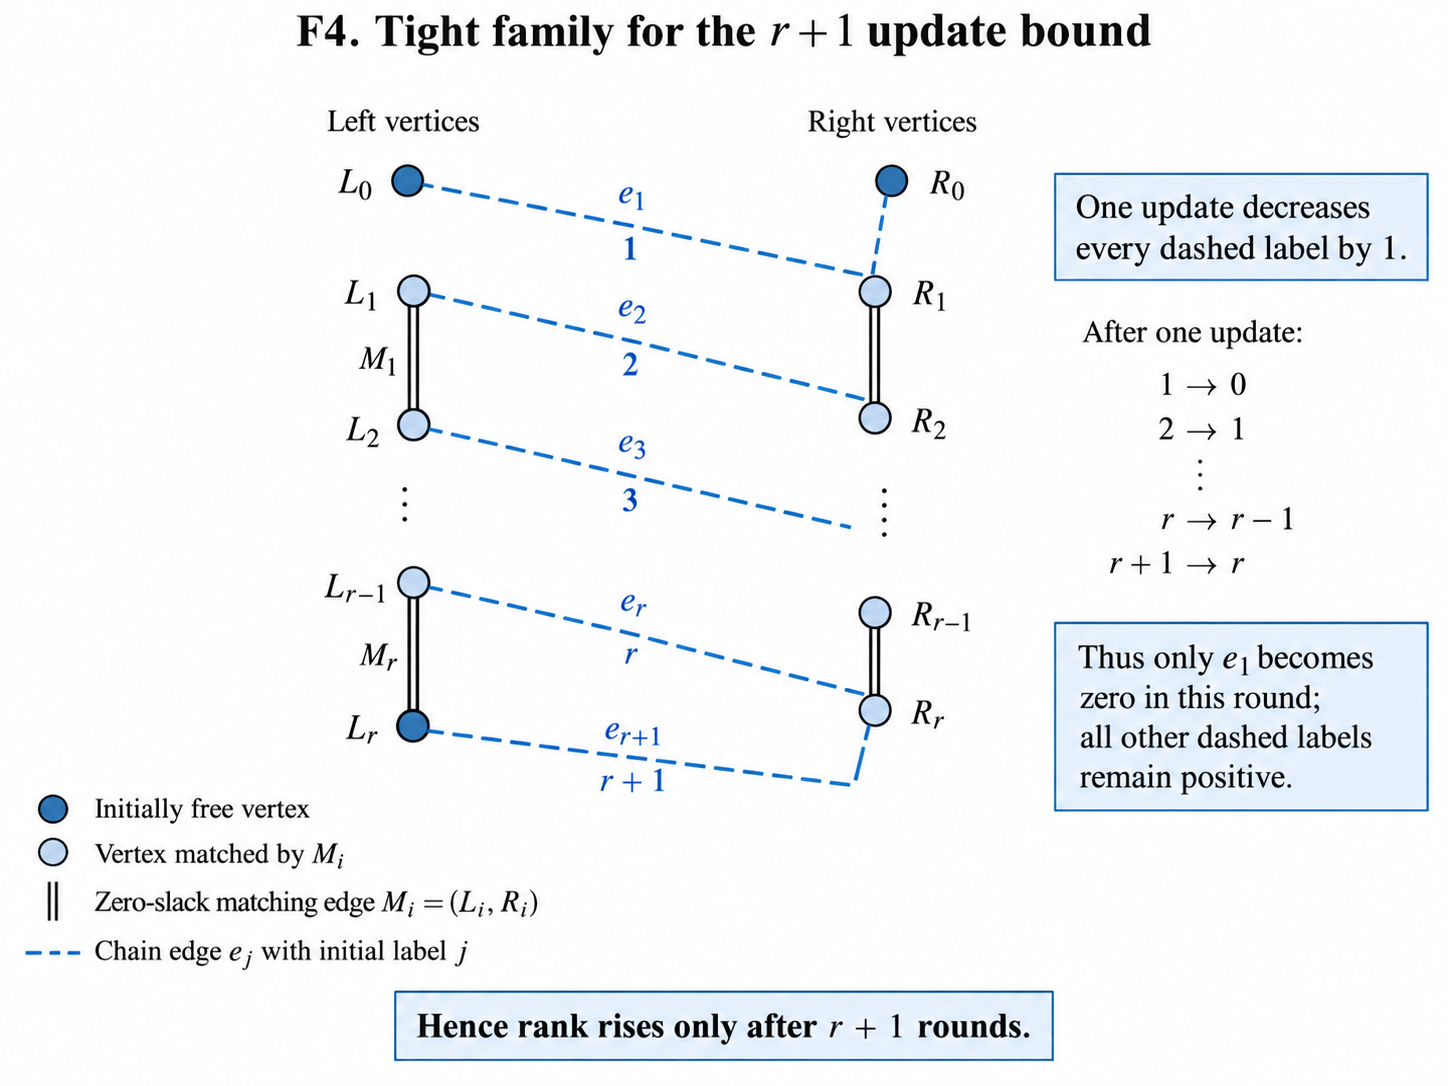
\includegraphics[width=0.88\textwidth]{fig/4.png}
  \caption{The family of Remark~\ref{rem:tight}.  Solid double lines are the
  zero-slack matching, dashed lines are the chain edges with their slacks.  One
  application of $U_r$ lowers every dashed slack by exactly one, so the rank
  rises only at the $(r+1)$-st.}
  \label{fig:tight}
\end{figure}

\begin{remark}[The bound $r+1$ is attained]
\label{rem:tight}
Take $L_0,\ldots,L_r$ and $R_0,\ldots,R_r$, so $n=r+1$.  Let $D$ vanish on the
edges $L_iR_i$ for $1\le i\le r$, let $D_{e_i}=i$ on $e_i=L_{i-1}R_i$ for
$1\le i\le r$, let $D_{e_{r+1}}=r+1$ on $e_{r+1}=L_rR_0$, and let $H$ have no
other edges.  The zero graph has rank $r$.  Since $L_0$ meets only $e_1$, the
chain $e_1,\ldots,e_{r+1}$ is the unique perfect matching, so $\tau=r+1$, and an
$r$-matching avoiding $L_k$ must route $L_0,\ldots,L_{k-1}$ along the chain and
the rest along zero edges, so $\lambda_{L_k}=k$ and $\mu_{R_j}=j$ for
$j\ge1$ while $\mu_{R_0}=r+1$.  One update therefore gives
\[
  L_iR_i:\ 0-(r{+}1{-}i)+(r{+}1{-}i)=0,
  \qquad
  e_i:\ i-(r{+}2{-}i)+(r{+}1{-}i)=i-1,
\]
\[
  e_{r+1}:\ (r{+}1)-1+0=r,
\]
so every chain slack drops by exactly one, only $e_1$ becomes zero, the rank
stays $r$ and $S$ grows by one vertex.  The new state is the same family with
$r$ decreased, and the augmenting path appears only at the $(r+1)$-st
application.  The count in Theorem~\ref{thm:terminate} is therefore attained,
and no sharper analysis of $U_r$ shortens \eqref{eq:schedule}.
\end{remark}

\begin{proof}[Proof of Theorems~\ref{thm:main} and \ref{thm:main-support}]
Initialize $\mu=\min_{e}w_e$, $D_e=w_e-\mu$, $p_i=\mu$ and $q_j=0$, so
\eqref{eq:dual} holds with $D\ge0$.  Run the schedule \eqref{eq:schedule},
updating $D\mapsto U_rD$ together with $p_i\mapsto p_i+a_i$ and
$q_j\mapsto q_j-c_j$, which preserves $D_{ij}=w_{ij}-p_i-q_j$ exactly.
Lemma~\ref{lem:feasible} preserves $D\ge0$.  The rank of the zero graph is at
least $0$ initially, and Theorem~\ref{thm:terminate} gives rank at least $r+1$
after stage $r$, so after stage $n-1$ the zero graph has a perfect matching.
Output $z=\sum_ip_i+\sum_jq_j$, which equals $\Opt_H(w)$ by \eqref{eq:dual} and
the argument after Theorem~\ref{thm:main-support}.

The schedule has $n(n+1)/2$ updates.  One update is one application of
Theorem~\ref{thm:compiler} to the vector of the $N=2n$ observables
\eqref{eq:observables}, which Proposition~\ref{prop:observer} computes by a
single Boolean circuit of size $s=O(n^{2}m)$.  With $m\le n^{2}$ that is
$s=O(n^{4})$, so \eqref{eq:compiler-size} gives $O(n^{4}m+m^{2})$ gates per
update and $O(n^{6}m+n^{2}m^{2})$ for the schedule.  With $m\le n^{2}$ this is
$O(n^{8})$.  Every index is a function of $(n,E)$ alone, so
the family is uniform.  Negating the inputs and the output turns the minimum
into the maximum at the cost of $m+1$ subtractions.
\end{proof}

\subsection{What the circuit can select}
\label{sec:selectors}

Theorem~\ref{thm:main-support} returns a dual pair and not a matching.  That is
forced, and the reason is worth stating, because it also says what can be
returned instead.

\begin{proposition}[Primal and dual selectors]
\label{prop:selectors}
Let $n\ge2$.
\begin{enumerate}
  \item There is no continuous map $W\mapsto x(W)$ from $\mathbb R^{n\times n}$
        to the Birkhoff polytope with $\langle W,x(W)\rangle=\Assign_n(W)$ for
        every $W$, even allowing $x(W)$ to be fractional.
  \item There is a continuous piecewise linear map $W\mapsto(p(W),q(W))$ that is
        dual optimal at every $W$, computed by a circuit of size $O(n^{8})$ over
        $\max,+,-,0$, and it may be normalized so that $q_1\equiv0$.
\end{enumerate}
\end{proposition}

\begin{proof}
(1)  Put $M_0=\{(i,i):1\le i\le n\}$ and
$M_1=\{(1,2),(2,1)\}\cup\{(i,i):i\ge3\}$, let $W^{0}$ be $0$ on
$M_0\cup M_1$ and $1$ elsewhere, and let $V$ be $+1$ on $M_0\setminus M_1$,
$-1$ on $M_1\setminus M_0$ and $0$ elsewhere.

The edges of weight $0$ in $W^{0}$ are $(i,i)$ for $i\ge3$ together with the
four edges between $\{1,2\}$ and $\{1,2\}$.  A perfect matching of cost $0$ must
use $(i,i)$ at every row $i\ge3$ and must match rows $1,2$ into columns $1,2$, so
there are exactly two of them, $M_0$ and $M_1$, and $\Assign_n(W^{0})=0$.

A perfect matching meets rows $1$ and $2$ once each, so it uses at most two
edges of the support of $V$ and $|\langle V,\chi_M\rangle|\le2$ for every $M$.
For $0<s<1/4$ the costs are
\[
  \begin{array}{lcc}
    \toprule
    & \langle W^{0}+sV,\chi_M\rangle & \langle W^{0}-sV,\chi_M\rangle\\
    \midrule
    M=M_1 & -2s & +2s\\
    M=M_0 & +2s & -2s\\
    \text{any other } M & \ge1-2s>1/2 & \ge1-2s>1/2\\
    \bottomrule
  \end{array}
\]
so $M_1$ is the unique optimum at $W^{0}+sV$ and $M_0$ is the unique optimum at
$W^{0}-sV$.  In both cases the optimal face is a single vertex, so an exact
optimal $x(W)$, fractional or not, equals $\chi_{M_1}$ on one side of $s=0$ and
$\chi_{M_0}$ on the other, and its two one-sided limits differ.

(2)  Theorem~\ref{thm:main-support} produces $p$ and $q$ through a circuit over
$\max,+,-,0$, so they are continuous and piecewise linear, and \eqref{eq:dual}
together with the zero-slack perfect matching makes them dual optimal.  For the
normalization, replace $p_i$ by $p_i+q_1$ and $q_j$ by $q_j-q_1$: every slack
$w_{ij}-p_i-q_j$ and the value $\sum_ip_i+\sum_jq_j$ are unchanged, and
$q_1$ becomes $0$.  This costs $2n$ further gates.
\end{proof}

Hertrich and Sering~\cite{hertrich-sering25} observe the corresponding obstacle
for spanning trees, where a network cannot return the indicator vector of a tree.
Part (1) says the obstruction survives relaxation: not even a point of the
optimal face can be chosen continuously.  What can be returned continuously is
the whole optimal face.

\begin{corollary}[The optimal face]
\label{cor:optimal-face}
For $ij\in E(K_{n,n})$ put
\begin{equation}
  \gamma_{ij}(W)=w_{ij}+\Assign_{n-1}\bigl(W_{\hat\imath,\hat\jmath}\bigr)-\Assign_n(W),
  \label{eq:forced-gap}
\end{equation}
where $W_{\hat\imath,\hat\jmath}$ deletes row $i$ and column $j$.  Then
$\gamma\ge0$, the map $W\mapsto\gamma(W)$ is continuous and piecewise linear and
is computed by a circuit of size $O(n^{10})$ over $\max,+,-,0$, and
\[
  \gamma_{ij}(W)=0
  \iff
  \text{some optimal perfect matching uses } ij .
\]
Consequently the optimal face of the Birkhoff polytope at $W$ is
$\{X\in B_n: X_{ij}=0 \text{ whenever } \gamma_{ij}(W)>0\}$.
\end{corollary}

\begin{proof}
The quantity $w_{ij}+\Assign_{n-1}(W_{\hat\imath,\hat\jmath})$ is the least cost
of a perfect matching through $ij$, so $\gamma_{ij}\ge0$ with equality exactly
when some optimum uses $ij$.  Running the circuit of Theorem~\ref{thm:main} once
per pair gives the size.  For the face, $\gamma_{ij}=0$ implies $ij$ is tight at
any optimal dual, so every perfect matching inside the graph
$\{\gamma=0\}$ has all edges tight and is optimal, while every optimal matching
lies in that graph.  Birkhoff's theorem applied to that subgraph identifies the
doubly stochastic matrices supported in it with the convex hull of those
matchings.
\end{proof}

An exclusion gap behaves symmetrically: $\eta_e=\Opt_H(H\setminus e)-\Opt_H(H)$
is positive exactly when $e$ lies in every optimal matching.

\section{Separation and bounded-cost robustness}
\label{sec:separation}

\paragraph{What is quoted, and the sign convention.}
Jerrum and Snir~\cite{jerrum-snir82} prove that monotone arithmetic circuits for
the permanent, equivalently pure tropical circuits for $\Assign_n$ correct at all
real weights, need $2^{\Omega(n)}$ gates.  Hertrich and
Stargalla~\cite{hertrich-stargalla26} prove that positive-scalar tropical
circuits for the support function of the Birkhoff polytope need $2^{\Omega(n)}$
addition gates, where $n$ counts the vertices on one side and not the $n^{2}$
inputs.

The first statement is already about the minimum and transfers directly.  The
second is about a maximum, $\max_M\langle x,\chi_M\rangle$, while \eqref{eq:opt}
is a minimum, so one syntactic step is needed.  Given a circuit
$C$ over $\min$, $+$, positive scalars and $0$, let $C^{\vee}$ be the circuit
obtained by replacing every $\min$ gate by a $\max$ gate and changing nothing
else.  Induction on the gates gives
\begin{equation}
  C^{\vee}(x)=-C(-x)
  \qquad\text{for every } x,
  \label{eq:conjugation}
\end{equation}
since negation commutes with $+$ and with multiplication by a positive scalar,
fixes the constant $0$, and exchanges $\min$ with $\max$.  The rewriting adds no
gate, introduces no subtraction, and preserves the number of addition gates.  A
positive-scalar circuit computing $\Opt_{K_{n,n}}$ therefore yields one of the
same size computing the support function of the Birkhoff polytope, so part (2)
of Theorem~\ref{thm:separation} follows from the quoted bound through
\eqref{eq:conjugation}.  On the upper side the corresponding remark is the last
sentence of the proof of Theorem~\ref{thm:main}: negating the inputs and the
output turns \eqref{eq:opt} into the maximum at the cost of $m+1$ subtractions.

\paragraph{What we add.}
Both quoted bounds assume exact computation at unbounded real weights.  Neither
assumption carries the bound.  The proofs are in Appendix~\ref{app:lower}, for an
arbitrary graph rather than for $K_{n,n}$ alone, and in the larger models that
admit arbitrary finite real constant leaves; the chain is described here.

Let $H$ be a graph with a perfect matching on $N=|V(H)|\ge4$ vertices, write
$V=V(H)$, and let $\mathsf T=\{0,1,2\}$.  An output parse of a circuit
$\mathcal G$ selects one
child at each $\min$ gate, both at each $+$ gate and the unique child at each
scalar gate, and has a constant $\kappa_P$ and an exponent
$\alpha_P\in\mathbb R^{E}_{\ge0}$ with
$\mathcal G(w)=\min_P(\kappa_P+\langle\alpha_P,w\rangle)$.

\begin{lemma}[Five probes pin the canonical parses]
\label{lem:pin}
Suppose $|\mathcal G(w)-\Opt_H(w)|\le\varepsilon$ on $\mathsf T^{E}$, and either
$\mathcal G$ is pure tropical with $\varepsilon<1/2$, or $\varepsilon=0$.  Then
every output parse has $\kappa_P\ge-\varepsilon$, and for every $M\in\PM(H)$
there is an output parse $P_M$ with $\alpha_{P_M}=\chi_M$ and
$|\kappa_{P_M}|\le\varepsilon$.
\end{lemma}

The probes are the zero vector, $\mathbf1$, $2\cdot\mathbf1$, the vector that is
$1$ on $M$ and $2$ off $M$, and, for each vertex, the vector that is $2$ on its
incident edges and $0$ elsewhere.  The first four force the exponent off $M$ to
vanish and the constant to be small; the last force every vertex to carry mass
at least $1$, which pins the exponent on $M$.  At $\varepsilon=0$ no step uses
integrality, so the lemma serves both models.

From here the two models diverge.  In the pure model integrality turns three
estimates into exact statements, each needing $2\varepsilon<1$, and the tolerance
$1/2$ is where a single unit of an integer exponent stops being absorbable by
the error.  In the scalar model the exponent masses are fractional, and the
scope of a gate is recovered instead from the inequality $\deg_v(\alpha_P)\ge1$,
valid at every vertex for every parse of constant $0$, applied to both cross
substitutions at a gate.

\begin{lemma}[The scope of a gate is a vertex set]
\label{lem:scope}
Under the hypotheses of either part of Theorem~\ref{thm:robust}, every gate $h$
occurring in the parses $P_M$ carries a set $V_h\subseteq V$, independent of
$M$, such that the exponent of the subtree at $h$ has support exactly $M[V_h]$,
and $M[V_h]$ is a perfect matching of $H[V_h]$.  In the pure model that exponent
is $\chi_{M[V_h]}$; in the positive-scalar model its coefficients may be
fractional, and only the support is pinned.
\end{lemma}

\begin{lemma}[Capacity]
\label{lem:rect}
Let $D_h$ be the set of matchings assigned to a gate $h$ with scope $V_h$.  Then
$M\mapsto(M[V_h],M[V\setminus V_h])$ is injective on $D_h$, so
$|D_h|\le|\PM(H[V_h])|\cdot|\PM(H[V\setminus V_h])|$.
\end{lemma}

A parse leaf is an edge literal and covers two vertices, so $|V_h|$ is
subadditive at $+$ gates, equals $N$ at the root and is at most $2$ at a leaf.
Descending to the child of larger $|V_h|$ produces a gate with
$N/3<|V_h|\le2N/3$, and that gate is a child of a $+$ gate, so at most
$2|\mathcal G_+|$ of them occur.  With
\[
  s(H)=\max\bigl\{\,|\PM(H[V_1])|\cdot|\PM(H[V_2])|:\ V_1\sqcup V_2=V,\
  N/3<|V_1|\le2N/3\,\bigr\},
\]
Lemma~\ref{lem:rect} gives $|\mathcal G_+|\ge|\PM(H)|/(2\,s(H))$, and
Corollary~\ref{cor:families} evaluates the ratio at $\binom{n}{\lceil
n/3\rceil}$ for $K_{n,n}$ and for $K_{2n}$, both at $n\ge2$.  The hypothesis
$N\ge4$ is used once, in the descent: a leaf covers two vertices, so a node of
scope at most $2N/3$ exists only when $2\le2N/3$.  At $N=2$ the bound fails and
nothing is asserted, as it must be, since the single-edge graph is computed by
one input leaf and no addition gate.

Bipartiteness plays no role in any of this.  The complete-graph case is the one
that Section~\ref{sec:frontier} uses, since it shows that the obstacle removed
by Theorem~\ref{thm:main} on bipartite supports is still standing, at bounded
costs and under a constant tolerance, on general graphs.

\paragraph{Where the power sits.}
The comparison sharpens once the placement of the sign is separated from its
presence.  Binary subtraction adds nothing beyond unary negation, since
$x-y=x+(0-y)$, so the models differ only by whether the single scalar $-1$ is
available and where it may be used.  Three placements give three answers.

\begin{equation}
  \begin{array}{ll}
    \text{arbitrary positive scalars, anywhere} & 2^{\Omega(n)}\\[2pt]
    \text{negation at the input gates only} & 2^{\Omega(n)}\\[2pt]
    \text{one subtraction, at the output gate} & O(n^{8})
  \end{array}
  \label{eq:three-levels}
\end{equation}

The first line is Theorem~\ref{thm:robust}(2) together with
\cite{hertrich-stargalla26}.  The middle line is not ours: Jukna, Seiwert and
Sergeev~\cite{jukna-seiwert-sergeev20} prove that admitting the tropical
reciprocals $-w_e$ alongside the inputs $w_e$ shrinks a $(\min,+)$ circuit by at
most a quadratic factor, so an exponential bound survives it.  Our own argument
does not reach that line, because with $-w_e$ available a parse exponent lies in
$\mathbb Z^{E}$ rather than $\mathbb Z^{E}_{\ge0}$ and Step 2 of
Lemma~\ref{lem:pin-full} fails.  The third line is Theorem~\ref{thm:main}
together with Proposition~\ref{prop:normal-form} below.

\begin{proposition}[Cancellation at the output is already everything]
\label{prop:normal-form}
Let $\sigma$ be $\min$ or $\max$.  Every circuit of size $s$ over $\sigma$, $+$,
$-$ and the constant $0$ can be rewritten as $A-B$, where $A$ and $B$ are
circuits over $\sigma$, $+$ and the constant $0$ with $|A|+|B|\le8s$.
The two bases are interchangeable, since
$\max(a,b)=a+b-\min(a,b)$ and $\min(a,b)=a+b-\max(a,b)$ cost three gates each.
Consequently
\begin{equation}
  \Assign_n=A_n-B_n,
  \qquad
  A_n,B_n \text{ over } \min,+,0,
  \qquad
  |A_n|+|B_n|=O(n^{8}).
  \label{eq:normal-form}
\end{equation}
\end{proposition}

\begin{proof}
Carry every gate $g$ as a pair $(g^{+},g^{-})$ with $g=g^{+}-g^{-}$.  An input
$w_e$ takes $(w_e,0)$ and the constant $0$ takes $(0,0)$.  For the gates,
\[
  a+b:\ (a^{+}{+}b^{+},\ a^{-}{+}b^{-}),
  \qquad
  a-b:\ (a^{+}{+}b^{-},\ a^{-}{+}b^{+}),
\]
\[
  \sigma(a,b):\ \bigl(\sigma(a^{+}{+}b^{-},\,b^{+}{+}a^{-}),\ a^{-}{+}b^{-}\bigr),
\]
the last because $\sigma$ commutes with adding the constant $a^{-}{+}b^{-}$ to
both arguments.  Each gate contributes at most four new gates, and the two nodes
$g^{+},g^{-}$ are shared by all successors, so one list of at most $4s$ gates
carries every pair on a directed acyclic graph, and $A$ and $B$ read their
outputs from it.  The output pair gives $A-B$.  For
\eqref{eq:normal-form}, convert the circuit of Theorem~\ref{thm:main} to the
$\min$ basis at a factor of three and then normalize.
\end{proof}

The observation is due to Jukna, Seiwert and
Sergeev~\cite{jukna-seiwert-sergeev20}; the proof above is included because the
bound is used here on circuits with unbounded fan-out.

As a network this is a maxout network with $O(s)$ units and every weight in
$\{-1,0,1\}$.  So the distinction that matters is not between the inside of a
circuit and its output.  Supplying signs in advance, at the inputs, is
exponentially weak, while one cancellation at the output is already the full
strength of the model.

\begin{corollary}[Monotone against general, on the matching polytope]
\label{cor:monotone-separation}
Write $\nnc(P)$ for the least number of units of a maxout network computing the
support function of a polytope $P$, and $\mnnc(P)$ for the same quantity over
monotone networks and input-convex networks.  For the Birkhoff polytope
$P_{\mathrm{PERM}}$,
\[
  \mnnc(P_{\mathrm{PERM}})=2^{\Omega(n)},
  \qquad
  \nnc(P_{\mathrm{PERM}})=O(n^{8}).
\]
\end{corollary}

\begin{proof}
The lower bound is Hertrich and Stargalla~\cite{hertrich-stargalla26}.  For the
upper bound, apply \eqref{eq:conjugation} to the circuit of
Theorem~\ref{thm:main} to obtain one of the same size for the support function,
then convert gates to units.
\end{proof}

Hertrich and Stargalla obtain such a separation for directed spanning trees,
where a polynomial-size general construction was already available, and record
the matching case as open for want of one.  Hertrich and
Loho~\cite{hertrich-loho26} ask more generally whether $\nnc(P)$ can be bounded
polynomially in the extension complexity $\mathrm{xc}(P)$; since
$\mathrm{xc}(P_{\mathrm{PERM}})=O(n^{2})$, the Birkhoff polytope is one polytope
where it can.

\paragraph{Three questions of Jukna, Seiwert and Sergeev.}
The tropical permanent is
$\mathrm{Per}_n(x)=\min_M\sum_{e\in M}x_e$ over the perfect matchings of
$K_{n,n}$, which is $\Assign_n$.  Three consecutive questions
of~\cite{jukna-seiwert-sergeev20} are answered by the results above.

\begin{corollary}
\label{cor:jss}
\begin{enumerate}
  \item $\mathrm{Per}_n$ has $(\min,+,-)$ circuits of size $O(n^{8})$.
  \item $\operatorname{Size}_{\min,+,\max}(\mathrm{Per}_n)\ge2^{n^{1/3-o(1)}}$,
        so the $(\min,+,\max)$ against $(\min,+,-)$ gap is exponential against
        polynomial.
  \item $\operatorname{Lat}(\Lambda_n)\ge2^{n^{1/3-o(1)}}$ while
        $\operatorname{STrop}(\Lambda_n)=O(n^{6})$, so the $(\min,\max)$ against
        $(\min,+,-)$ gap is exponential against polynomial, and subtraction helps
        for a bottleneck problem.
\end{enumerate}
\end{corollary}

\begin{proof}
(1) is Theorem~\ref{thm:main} with the basis conversion of
Proposition~\ref{prop:normal-form}.  For (2), \cite{jukna-seiwert-sergeev20}
prove that a $(\min,+,\max)$ circuit of size $s$ for a minimization problem
yields a monotone Boolean circuit of size $s$ for its Boolean version, which for
$\mathrm{Per}_n$ is $\textsc{Match}_n$; substituting~\cite{cgrss26} for
Razborov~\cite{razborov85} in their corollary gives the stated bound, and (1)
gives the other side.  (3) is Corollary~\ref{cor:bottleneck}.
\end{proof}

Razborov's $n^{\Omega(\log n)}$ already makes the gaps in (2) and (3)
super-polynomial, so the answers do not depend on~\cite{cgrss26}, which sharpens
them to exponential.  By Proposition~\ref{prop:normal-form} each upper bound
here is attained with one subtraction gate, placed at the output.

\begin{remark}[The hypotheses are not interchangeable]
\label{rem:not-combinable}
Part (1) of Theorem~\ref{thm:robust} uses integrality twice: to turn an
$\ell_1$ estimate on exponents into an exact indicator, and to turn a degree
estimate into an exact degree.  A positive scalar gate destroys both, and the
tolerance in part (2) is therefore zero.  A common statement covering a
tolerance and positive scalars at the same time is not available here, and
Section~\ref{sec:frontier} records why.
\end{remark}

\section{Verification and trust boundaries}
\label{sec:verification}

The construction is implemented, and the implementation is audited at four
levels that prove different quantifiers.  We state them separately because a
large count at one level does not substitute for another.

\begin{enumerate}
  \item \emph{General proof.}  Sections~\ref{sec:amplitude} and
        \ref{sec:circuit} and Appendix~\ref{app:graph} carry
        the quantifier over every $n$ and every $w\in\mathbb R^{E}$.  This is the
        only level that does.
  \item \emph{Fixed-dimension certificate over all reals.}  The complete
        generated circuit at $n=2$ is replayed over a covering family of closed
        polyhedral cones, $24$ order chambers and $40$ terminal cones, each
        maximum choice justified by an explicit rational nonnegative combination
        and each leaf carrying a symbolic primal-dual certificate.  This covers
        every real $2\times2$ input, including ties, relative to a small replay
        program that imports no generator, matching routine or solver.  It does
        not extend the dimension quantifier.
  \item \emph{Symbolic bounded-dimension checks.}  Across the $247$ feasible
        supports at $n=3$, the one-step update is an integer linear map in the
        successive gaps, and exact integer coefficient checks establish
        Lemma~\ref{lem:feasible} and Theorem~\ref{thm:progress} on all
        $2{,}647{,}507$ order cones rather than at sampled magnitudes.
  \item \emph{Finite exhaustive checks.}  The generated Boolean observer is
        compared with independent minimum-cover enumeration and an independent
        rank oracle on all $2^{25}$ bipartite graphs at $n=5$.  The generated
        signed circuit is evaluated with overflow-checked integer arithmetic on
        the complete grid $\{-1,0,1\}^{9}$ at $n=3$ and the complete grid
        $\{-1,0\}^{16}$ at $n=4$, with the value, the dual identities
        \eqref{eq:dual}, the slack signs and the zero perfect matching checked
        against a separately written reference.
\end{enumerate}

Three controls are recorded in Appendix~\ref{app:verify} rather than omitted:
twelve deliberate corruptions of the certificates, all rejected; states in which
a zero edge disappears, so that no proof step assumes the zero graph is monotone
under the update; and one monolithic query that returned unknown and is not
counted as evidence.

\section{Scope and the non-bipartite frontier}
\label{sec:frontier}

The construction uses bipartiteness in one place, and it uses it twice over.
Equation~\eqref{eq:cover} is the K\H{o}nig equality between the maximum matching
size and the minimum vertex cover size, and the canonical two-sided reachable
pair $(S,T)$ is the minimum cover it produces.  Step 1 of
Theorem~\ref{thm:progress} needs that cover to meet every edge of a maximum
matching exactly once, which is what makes the potential update leave old zero
edges at zero, and Step 3 needs the deficiency count $|S_0|-|T_0|=n-r$ to produce
a boundary edge.  On general graphs the equality fails at the triangle, where
$\nu=1$ and the minimum vertex cover has size $2$, so neither step survives as
written.

\begin{problem}
Do minimum-weight perfect-matching value functions on general graphs admit
polynomial-size signed tropical circuits over all real edge weights?
\end{problem}

Our construction resolves the bipartite case.  Extending it requires a
replacement for the canonical-cover progress mechanism, with a dual object that
has a fixed index set.  The odd-set duals $z_S$ of the blossom algorithm do not
have one, but their semantics may: a reduced slack depends on $z$ only through
$U_{uv}=\sum_{S\supseteq\{u,v\}}z_S$, and with $d_v=\sum_{S\ni v}z_S$ and
$t=\sum_Sz_S$ the dual objective contributes
$\sum_S\tfrac{|S|-1}2z_S=\tfrac12(\sum_vd_v-t)$.  Both the slacks and the
objective therefore factor through the polynomial-dimensional triple
$(U,d,t)$.  For a laminar family with positive weights the sets containing a
fixed pair form a chain, so $U$ is a hierarchical pairwise similarity, and when
the cumulative levels are distinct the sets $\{v:U_{uv}\ge\theta\}$ recover the
family as $\theta$ decreases.  A vanishing weight collapses one level of the
hierarchy, which is where an amplitude would have to absorb the ambiguity.  What
is missing is the step from recovering the family to driving the next update,
and a reading of blossom formation and dissolution as threshold data.

The obstacle on general graphs is not an artifact of the question being posed at
unbounded weights.  Appendix~\ref{app:lower} works over an arbitrary graph, and
Corollary~\ref{cor:families} applies it to $K_{2n}$: every pure tropical circuit
correct within an additive $\varepsilon<1/2$ at edge weights in $\{0,1,2\}$, and
every positive-scalar tropical circuit exact at those weights, needs
$\tfrac12\binom{n}{\lceil n/3\rceil}$ addition gates for minimum-weight perfect
matching on $2n$ vertices.  The two sides of the problem are therefore stated
over the same class.  For general graphs the barrier stands at bounded costs and
under a constant tolerance, and what is missing is a construction, not a sharper
bound.

\paragraph{Three further questions.}
The construction spends threshold integrals, and Section~\ref{sec:amplitude}
compiles exactly those.  The schedule \eqref{eq:schedule} uses $n(n+1)/2$
updates because Theorem~\ref{thm:progress} moves the rank only after the
reachable set has been exhausted, and a single update per stage would give
$n$ of them.  Such an update exists classically: with $d_v$ the shortest
alternating path distances from the unmatched left vertices, forward edges
weighted by $D$ and matched edges by $0$, and $\delta$ the least $d_j$ over
unmatched $j$, the potentials $a_i=(\delta-d_i)_+$ and $c_j=(\delta-d_j)_+$
preserve \eqref{eq:dual}, keep $D\ge0$, and make a whole augmenting path tight
at once.  Its ingredients are not threshold integrals: $\delta$ is the least
cost of an $(r+1)$-matching in the reduced costs and $d_i$ the least cost of an
$r$-matching avoiding $i$, so reading them off is again a minimum-cost matching
computation.

Existence is not the open part.  Fixed-cardinality matching reduces to perfect
matching: given $H$ and $k$, adjoin $n-k$ vertices to each side, join the new
left vertices to $R$ and the new right vertices to $L$ at cost $0$, and leave the
two new sides unjoined.  A perfect matching of the enlarged graph, which has
$2n-k$ vertices per side, must send all $n-k$ new left vertices into $R$ and all
$n-k$ new right vertices into $L$, hence uses exactly $k$ original edges, so its
value is the least cost of a $k$-matching of $H$.  Theorem~\ref{thm:main-support}
therefore already gives polynomial-size circuits for $\delta$ and for every
$d_i$.  What that argument does not give is a construction: it would call one
assignment-scale circuit per distance, $n+1$ of them per rank stage, so it
cannot shorten \eqref{eq:schedule} and, used as a proof of
Theorem~\ref{thm:main}, it would be circular.

\begin{problem}
Does the whole vector of shortest alternating path distances admit a direct
realization substantially smaller than solving the auxiliary assignment
instances above?  A realization inside the compiler of
Section~\ref{sec:amplitude} is ruled out by Remark~\ref{rem:not-braid}.
\end{problem}

Finally, Theorem~\ref{thm:robust} tolerates an additive error in the pure model
and none in the positive-scalar model.  The asymmetry is not a missing constant.
At $\varepsilon=0$ the cross constants at a gate vanish exactly, which pins the
scale of a subtree; at $\varepsilon>0$ they are only $O(\varepsilon)$ while the
context scalar is unbounded, and inserting the pair $x\mapsto\eta x\mapsto
\eta^{-1}x$ rescales every subtree without changing the function or the gate
count.

\begin{problem}
Find a scale-invariant gate invariant for positive-scalar tropical circuits, and
with it an exponential lower bound for $\Assign_n$ under some constant additive
error at costs in $\{0,1,2\}$.
\end{problem}

\paragraph{Depth.}
The schedule is the only sequential part of the construction.  With the
$\mathsf{NC}$ observer of Remark~\ref{rem:depth-separation}, one update has depth
$\operatorname{polylog}(n)$, so the whole circuit has size $n^{O(1)}$ and depth
$O(n^{2}\operatorname{polylog}n)$, and a positive answer to the first problem
above would bring it to $O(n\operatorname{polylog}n)$.

\paragraph{Outside the scope.}
The results above concern gate count under exact real arithmetic at a support
fixed in the circuit.  Floating-point stability, circuit depth, running time
against the Hungarian method in practice, the algebraic permanent, supports
supplied at runtime, and minimum-cost flow with real supplies lie outside them.

\bibliographystyle{plain}
\bibliography{references}


\appendix

\section{Bipartite preliminaries, the observer, and the gate count}
\label{app:graph}

Throughout, $H=(L,R,E)$ is bipartite with $|L|=|R|=n$ and $m=|E|$, and
$G\subseteq H$ is a subgraph on the same vertex set.  For a matching $M$ of $G$,
a vertex is $M$-free if no edge of $M$ meets it, and an $M$-alternating path
from an $M$-free left vertex uses edges outside and inside $M$ in turn, starting
outside.  Put
\[
  S(G)=\{\,i\in L:\ i \text{ is } M\text{-free, or reached by such a path}\,\},
  \qquad
  T(G)=N_G(S(G)).
\]

\begin{lemma}[Canonical cover]
\label{lem:canonical}
Let $M$ be a maximum matching of $G$.  Then
\begin{enumerate}
  \item every $j\in T(G)$ is matched by $M$, and its partner lies in $S(G)$;
  \item $|S(G)|-|T(G)|=n-\nu(G)$;
  \item $(L\setminus S(G))\cup T(G)$ is a minimum vertex cover of $G$;
  \item $S(G)=\{i\in L:\nu(G-i)=\nu(G)\}$, so $S(G)$ and $T(G)$ do not depend on
        the choice of $M$.
\end{enumerate}
\end{lemma}

\begin{proof}
(1)  Let $j\in T(G)$ be reached from $i\in S(G)$ along an edge $ij\notin M$.  If
$j$ were $M$-free, the alternating path to $i$ extended by $ij$ would be
$M$-augmenting, contradicting maximality.  Let $i'$ be the partner of $j$;
extending the path by $ji'$ puts $i'\in S(G)$.

(2)  By (1) the matching $M$ restricts to an injection $T(G)\to S(G)$.  Every
$i\in S(G)$ is either $M$-free or reached along an edge of $M$ from a vertex of
$T(G)$, because an alternating path arrives at a left vertex through a matching
edge.  Hence $S(G)$ is the disjoint union of the $M$-free left vertices, of
which there are $n-\nu(G)$, and the partners of $T(G)$.

(3)  Put $C=(L\setminus S(G))\cup T(G)$.  Then
\begin{align*}
  ij\in E(G),\ i\in S(G)
    &\ \Longrightarrow\ j\in N_G(S(G))=T(G)\subseteq C,\\
  ij\in E(G),\ i\notin S(G)
    &\ \Longrightarrow\ i\in L\setminus S(G)\subseteq C,\\
  \text{so $C$ is a vertex cover, and}
    &\ |C|=n-|S(G)|+|T(G)|\overset{(2)}{=}\nu(G),
\end{align*}
which is minimum because every vertex cover has at least $\nu(G)$ vertices.

(4)  If $i\in S(G)$, reversing the alternating path from an $M$-free left vertex
to $i$ produces a maximum matching leaving $i$ free, so $\nu(G-i)=\nu(G)$.
Conversely let $M'$ be a maximum matching leaving $i$ free.  If $i$ is $M$-free
then $i\in S(G)$ by definition.  Otherwise let $P$ be the component of
$M\triangle M'$ containing $i$, a path starting at $i$ with an edge of $M$.  If
$P$ ended with an edge of $M$ it would be $M'$-augmenting and $M'$ would not be
maximum, so $P$ ends with an edge of $M'$ at a vertex $v$ that is $M$-free.
Then $P$ has even length, so $v\in L$, and read from $v$ to $i$ it is
$M$-alternating from an $M$-free left vertex.  Hence $i\in S(G)$.  The
right-hand description does not mention $M$, and $T(G)=N_G(S(G))$ is determined
by $S(G)$.
\end{proof}

\begin{proposition}[Boolean observer]
\label{prop:observer}
For fixed $(n,E)$ there is a Boolean circuit $\Theta$ over $\wedge,\vee,\neg$
with $m$ inputs and $O(n^{2}m)$ gates which, on the adjacency bits of any
$G\subseteq H$, outputs the indicator vectors of $S(G)$ and $T(G)$ and, for each
$r<n$, the bit $\mathbf1[\nu(G)\le r]$.
\end{proposition}

\begin{proof}
The circuit keeps a bit $x_e$ for each $e\in E$, initially $0$, encoding a
matching, and runs $n$ rounds.  Write $g_e$ for the input bit of the edge $e$.

\emph{Reachability.}  With $x$ fixed, set $z^{(0)}_i=\neg\bigvee_{e\ni i}x_e$ for
$i\in L$ and $y^{(0)}_j=0$ for $j\in R$, and for $t<2n$ put
\[
  y^{(t+1)}_j=y^{(t)}_j\vee\bigvee_{ij\in E}\bigl(g_{ij}\wedge\neg x_{ij}\wedge z^{(t)}_i\bigr),
  \qquad
  z^{(t+1)}_{i}=z^{(t)}_{i}\vee\bigvee_{ij\in E}\bigl(g_{ij}\wedge x_{ij}\wedge y^{(t+1)}_j\bigr).
\]
One layer costs $O(m)$ gates and $2n$ layers saturate, so reachability costs
$O(nm)$ gates and returns the alternating reachable sets of the current $x$.

\emph{First discovery and parents.}  Layer bits are cumulative, so with
$y^{(-1)}=z^{(-1)}=0$ record
\[
  \widehat y^{(t)}_j=y^{(t)}_j\wedge\neg y^{(t-1)}_j,
  \qquad
  \widehat z^{(t)}_i=z^{(t)}_i\wedge\neg z^{(t-1)}_i ,
\]
so each vertex carries at most one first-discovery half-level.  Write
$\pi_u(c_1,\ldots,c_s)=c_u\wedge\bigwedge_{u'<u}\neg c_{u'}$ for the priority
encoder, which costs $O(s)$ gates with running prefixes of the negations, and
set
\begin{align*}
  \widehat y^{(t+1)}_j=1
    &\ \Longrightarrow\
    \mathrm{par}(j)=\pi\bigl(\,g_{ij}\wedge\neg x_{ij}\wedge z^{(t)}_i\,\bigr)_{i\in L},\\
  \widehat z^{(t+1)}_i=1
    &\ \Longrightarrow\
    \mathrm{par}(i)=\text{the $x$-partner of $i$} .
\end{align*}
Every candidate is masked in parallel over all $e\in E$, so no wire index
depends on a computed value.

\emph{Augmentation.}  A round succeeds if some $j\in R$ is reachable and
$x$-free; select the least such $j$ by $\pi$ and follow $\mathrm{par}$.  A parent
has strictly smaller first-discovery half-level, so the walk visits each vertex
at most once, reaches an $x$-free left vertex within $2n$ steps, and is a simple
$x$-alternating augmenting path.  Complement $x$ along it.

\emph{Output.}  A round succeeds exactly while the current matching is not
maximum, so $\mathbf1[\nu(G)\le r]$ is the negation of the success bit of round
$r+1$.  One further reachability pass returns $S(G)$, and
$T_j=\bigvee_{ij\in E}(g_{ij}\wedge S_i)$.  Every selection is a Boolean
function of the input bits, so the circuit is well defined.

\emph{Cost.}
\[
  \begin{array}{lcl}
    \toprule
    \text{reachability, } 2n \text{ layers at } O(m) & : & O(nm)\\
    \text{first discovery and parents} & : & O(nm)\\
    \text{selection and back-walk, } 2n \text{ steps at } O(m) & : & O(nm)\\
    \text{complementing } x & : & O(m)\\
    \midrule
    \text{one round} & : & O(nm)\\
    n \text{ rounds, plus } S \text{ and } T & : & O(n^{2}m)\\
    \bottomrule
  \end{array}
\]
\end{proof}

Since $m\le n^{2}$, the observer has $O(n^{4})$ gates.  Lemma~\ref{lem:lift}
lifts it at a constant factor, so one gap of one update costs $O(n^{4})$ gates
for the observer, $O(m)$ gates for the membership values of Lemma~\ref{lem:bit},
and $O(n)$ gates for the accumulation \eqref{eq:ac}.  With $m$ gaps and one
sorting network of $O(m\log^{2}m)$ comparators, one update costs
$O(n^{4}m+m^{2})$ gates, and the schedule \eqref{eq:schedule}, of $n(n+1)/2$
updates, costs
\[
  O\bigl(n^{6}m+n^{2}m^{2}\bigr)\ \text{ gates,}
  \qquad
  O(n^{8})\ \text{ when } m=n^{2},
\]
which is \eqref{eq:main-support} and \eqref{eq:main}.
\label{app:observer}
\label{app:count}

\section{Bounded-cost lower bounds}
\label{app:lower}

This appendix works over an arbitrary graph $H$ with a perfect matching on
$N\ge4$ vertices, not only over bipartite ones, and in the two models of
Definition~\ref{def:models} enlarged by arbitrary finite real constant leaves.
Write $V=V(H)$, $N=|V|$, $E=E(H)$, and let
$\chi_M\in\{0,1\}^{E}$ be the indicator of $M\in\PM(H)$.  For $\alpha\in\mathbb
R_{\ge0}^{E}$ and $v\in V$ put $\deg_v(\alpha)=\sum_{e\ni v}\alpha_e$ and
$\deg(\alpha)=\sum_e\alpha_e$, and let $e_M(v)$ be the edge of $M$ at $v$.  For
$U\subseteq V$, $H[U]$ is the induced subgraph and $M[U]$ the set of edges of
$M$ with both endpoints in $U$.  Costs are drawn from $\mathsf T=\{0,1,2\}$.

\begin{definition}[Splitting number]
\label{def:splitting}
A \emph{balanced bipartition} of $H$ is a pair $(V_1,V_2)$ of disjoint sets with
$V_1\cup V_2=V$ and $N/3<|V_1|\le 2N/3$.  Put
\[
  s(H)=\max\bigl\{\,|\PM(H[V_1])|\cdot|\PM(H[V_2])|\ :\ (V_1,V_2)
  \text{ a balanced bipartition}\,\bigr\}.
\]
\end{definition}

For a circuit $\mathcal G$ in one of the first two models of
Definition~\ref{def:models}, an \emph{output parse} is obtained by unfolding
$\mathcal G$ into a tree and retaining one child at each $\min$ gate, both
children at each $+$ gate and the unique child at each scalar gate.  A parse $P$
has a constant $\kappa_P\in\mathbb R$ and an exponent
$\alpha_P\in\mathbb R_{\ge0}^{E}$, integral in the pure model, with
\begin{equation}
  \mathcal G(w)=\min_P\bigl(\kappa_P+\langle\alpha_P,w\rangle\bigr).
  \label{eq:parse}
\end{equation}
For a node $h$ of a parse tree, $A^h$ and $\kappa^h$ denote the exponent and the
constant accumulated below $h$, and $\sigma^h>0$ the product of the scalars on
the path from $h$ to the root, so that $\alpha_P=\sigma^hA^h+B^h$ and
$\kappa_P=\sigma^h\kappa^h+\kappa^{B,h}$ for the context pair
$(B^h,\kappa^{B,h})$.  In the pure model $\sigma^h=1$.

\subsection{Five probes pin the canonical parses}

\begin{lemma}
\label{lem:pin-full}
Suppose $|\mathcal G(w)-\Opt_H(w)|\le\varepsilon$ for every $w\in\mathsf T^{E}$,
and that either $\mathcal G$ is pure tropical with $\varepsilon<1/2$, or
$\varepsilon=0$.  Then $\kappa_P\ge-\varepsilon$ for every output parse $P$, and
for every $M\in\PM(H)$ there is an output parse $P_M$ with
\[
  \alpha_{P_M}=\chi_M,
  \qquad
  |\kappa_{P_M}|\le\varepsilon .
\]
\end{lemma}

\begin{proof}
Five probes suffice: the zero vector, the all-ones vector $\mathbf1$, the
all-twos vector $2\cdot\mathbf1$, the vector $u^{M}$ that is $1$ on $M$ and $2$
off $M$, and, for each vertex $v$, the vector $y^{v}$ that is $2$ on the edges
at $v$ and $0$ elsewhere.  All five lie in $\mathsf T^{E}$.

\emph{Step 1: the probe values.}
$\Opt_H(0)=0$, $\Opt_H(\mathbf1)=N/2$ and $\Opt_H(2\cdot\mathbf1)=N$ because
every perfect matching has $N/2$ edges.  Every perfect matching uses exactly one
edge at $v$, so $\Opt_H(y^{v})=2$.  For $M'\in\PM(H)$,
\[
  \sum_{e\in M'}u^{M}_e
  =|M\cap M'|+2\,|M'\setminus M|
  =|M\cap M'|+2\bigl(\tfrac N2-|M\cap M'|\bigr)
  =N-|M\cap M'|
  \ \ge\ \tfrac N2 ,
\]
with equality exactly at $M'=M$, so $\Opt_H(u^{M})=N/2$.

\emph{Step 2: no mass off $M$.}
At $w=0$ we get $\min_P\kappa_P=\mathcal G(0)\ge-\varepsilon$.  Let $P_M$ attain
the minimum \eqref{eq:parse} at $u^{M}$, write $\kappa=\kappa_{P_M}$,
$A=\sum_{e\in M}(\alpha_{P_M})_e$ and $B=\sum_{e\notin M}(\alpha_{P_M})_e$.
Selection at $u^{M}$ and correctness at $\mathbf1$ give
\begin{equation}
  \kappa+A+2B\ \le\ \tfrac N2+\varepsilon,
  \qquad
  \kappa+A+B\ \ge\ \mathcal G(\mathbf1)\ \ge\ \tfrac N2-\varepsilon ,
  \label{eq:two-probes}
\end{equation}
the second because $\mathcal G(\mathbf1)$ is a minimum over all parses.
Subtracting, $B\le2\varepsilon$.  In the pure model $B$ is a nonnegative integer
and $2\varepsilon<1$, and at $\varepsilon=0$ it is a nonnegative real bounded by
$0$; either way $B=0$.

\emph{Step 3: the constant is small.}
Correctness at $2\cdot\mathbf1$ gives $\kappa+2A\ge N-\varepsilon$, while
\eqref{eq:two-probes} with $B=0$ gives $\kappa+A\le N/2+\varepsilon$.  Twice the
second minus the first yields $\kappa\le3\varepsilon$.

\emph{Step 4: every vertex carries mass at least one.}
Correctness at $y^{v}$ gives $\kappa+2\deg_v(\alpha_{P_M})\ge2-\varepsilon$, so
$\deg_v(\alpha_{P_M})\ge1-2\varepsilon>0$.  In the pure model the degree is an
integer, hence at least $1$; at $\varepsilon=0$ the displayed bound is already
$1$.  Since $B=0$, the only edge of the support at $v$ is $e_M(v)$, so
$(\alpha_{P_M})_{e_M(v)}\ge1$ for every $v$ and therefore $A\ge N/2$.

\emph{Step 5: the exponent is the indicator.}
From $\kappa\ge-\varepsilon$ and $\kappa+A\le N/2+\varepsilon$ we get
$A\le N/2+2\varepsilon$, which forces $A\le N/2$ in the pure model because $A$ is
an integer and $2\varepsilon<1$, and at $\varepsilon=0$ directly.  With Step 4,
$A=N/2$ and the $N/2$ coefficients on $M$, each at least $1$, sum to $N/2$, so
each equals $1$ and $\alpha_{P_M}=\chi_M$.  Finally
$\kappa=\mathcal G(u^{M})-N/2\in[-\varepsilon,\varepsilon]$.
\end{proof}

The argument uses integrality only in the pure model, and only to turn the three
bounds $B\le2\varepsilon$, $\deg_v\ge1-2\varepsilon$ and $A\le N/2+2\varepsilon$
into exact statements.  Each of them needs $2\varepsilon<1$, and
Theorem~\ref{thm:pure-full} below needs nothing weaker, which is why the
tolerance is $1/2$ throughout.

\subsection{The scope of a gate is a vertex set}

Both models reach the same structural conclusion, and the counting step is
common to them.  We isolate it first.

\begin{definition}[Vertex scope]
\label{def:vertex-scope}
For a node $h$ of the parse $P_M$ put
$V^h_M=\{v\in V:\deg_v(A^h_M)>0\}$.
\end{definition}

\begin{lemma}[Counting from a balanced scope]
\label{lem:count}
Let $\mathcal D$ be a family of output parses containing one parse $P_M$ for
every $M\in\PM(H)$.  Suppose that every circuit gate $h$ occurring in $\mathcal
D$ carries a set $V_h\subseteq V$ with $V^h_M=V_h$ for every $M$ using that
occurrence, and that $M[V_h]$ is a perfect matching of $H[V_h]$ for every such
$M$.  Suppose further that $|V^h_M|$ is subadditive at $+$ gates, unchanged at
$\min$ and scalar gates, equal to $N$ at the root and at most $2$ at a leaf.
Then, for $N\ge4$,
\[
  |\mathcal G_+|\ \ge\ \frac{|\PM(H)|}{2\,s(H)} .
\]
\end{lemma}

\begin{proof}
\emph{Step 1: a balanced gate.}
Fix $M$ and descend $P_M$ from the root, always to the child with the larger
value of $|V^{\cdot}_M|$, stopping at the first node $h(M)$ whose value is at
most $2N/3$.  The descent reaches one, because leaves have value at most $2$ and
$N\ge4$ gives $2\le2N/3$.  The root has value $N>2N/3$, so the descent is not
empty.
The parent of $h(M)$ has value greater than $2N/3$, and subadditivity makes the
larger child at least half the parent, so $|V^{h(M)}_M|>N/3$.  A $\min$ or
scalar gate does not change the value, so the first drop occurs at a child of a
$+$ gate, and $h(M)$ is such a child.  Hence $(V_{h(M)},V\setminus V_{h(M)})$ is
a balanced bipartition of $H$.

\emph{Step 2: a group is a product.}
Group the matchings by the circuit gate underlying $h(M)$; at most
$2|\mathcal G_+|$ gates occur as children of $+$ gates.  Let $D_h$ be one group
and $V_h$ its scope.  For $M\in D_h$ the set $M[V_h]$ is a perfect matching of
$H[V_h]$, so $M$ has no edge between $V_h$ and $V\setminus V_h$, and
$M=M[V_h]\cup M[V\setminus V_h]$.  The map
$M\mapsto(M[V_h],M[V\setminus V_h])$ is therefore injective on $D_h$, and
\[
  |D_h|\ \le\ |\PM(H[V_h])|\cdot|\PM(H[V\setminus V_h])|\ \le\ s(H).
\]

\emph{Step 3.}  Summing over the groups gives
$|\PM(H)|\le2|\mathcal G_+|\,s(H)$.
\end{proof}

\subsection{The pure model at constant tolerance}

\begin{theorem}
\label{thm:pure-full}
Let $N\ge4$ and let $\mathcal G$ be a pure tropical circuit with
$|\mathcal G(w)-\Opt_H(w)|\le\varepsilon$ for every $w\in\mathsf T^{E}$ and
$\varepsilon<1/2$.  Then $|\mathcal G_+|\ge|\PM(H)|/(2\,s(H))$.
\end{theorem}

\begin{proof}
\emph{Step 1: the canonical parses.}
Lemma~\ref{lem:pin-full} supplies, for every $M$, a parse $P_M$ with
$\alpha_{P_M}=\chi_M$ and $|\kappa_{P_M}|\le\varepsilon$, and gives
$\kappa_P\ge-\varepsilon$ for every output parse.

\emph{Step 2: subtree exponents are sub-matchings.}
For a node $h$ of $P_M$ we have $\alpha_{P_M}=A^h+B^h$ with both summands
nonnegative and integral, so $A^h=\chi_F$ for a unique $F=F^h_M\subseteq M$ and
$B^h=\chi_{M\setminus F}$.  So $V^h_M$ is the vertex set covered by
$F^h_M$, and $F^h_M=M[V^h_M]$ is a perfect matching of $H[V^h_M]$.

\emph{Step 3: cross constants.}
Let $h$ be a circuit gate with an occurrence in $P_M$ and one in $P_{M'}$.
Substituting the subtree of one occurrence into the context of the other gives
output parses $Q$ and $Q'$ with
$\kappa_Q+\kappa_{Q'}=\kappa_{P_M}+\kappa_{P_{M'}}\le2\varepsilon$ and
$\kappa_Q,\kappa_{Q'}\ge-\varepsilon$, hence
$-\varepsilon\le\kappa_Q\le3\varepsilon$.

\emph{Step 4: cross degrees.}
Evaluating at $w=2\cdot\mathbf1$ gives
$\kappa_Q+2\deg(\alpha_Q)\ge\mathcal G(2\cdot\mathbf1)\ge N-\varepsilon$, so
$\deg(\alpha_Q)\ge N/2-2\varepsilon$, and likewise for $Q'$.  Since
$\deg(\alpha_Q)+\deg(\alpha_{Q'})=\deg(\alpha_{P_M})+\deg(\alpha_{P_{M'}})=N$,
both lie in $[N/2-2\varepsilon,N/2+2\varepsilon]$.  They are integers and
$2\varepsilon<1$, so $\deg(\alpha_Q)=N/2$.

\emph{Step 5: the cross exponent is a perfect matching.}
Let $w_e=2\cdot\mathbf1[(\alpha_Q)_e=0]$, so $\langle\alpha_Q,w\rangle=0$ and
$\mathcal G(w)\le\kappa_Q\le3\varepsilon$.  If no perfect matching lay inside
$\operatorname{supp}\alpha_Q$, every perfect matching would meet an edge of
weight $2$, giving $\Opt_H(w)\ge2$ and forcing $3\varepsilon\ge2-\varepsilon$,
that is $\varepsilon\ge1/2$, which is excluded.  Hence some $N_0\in\PM(H)$
satisfies
$N_0\subseteq\operatorname{supp}\alpha_Q$, and
$|\operatorname{supp}\alpha_Q|\le\deg(\alpha_Q)=N/2=|N_0|$ forces
$\alpha_Q=\chi_{N_0}$.

\emph{Step 6: the scope is gate-determined.}
Step 5 says that $F^h_{M'}\cup(M\setminus F^h_M)$ is a perfect matching of $H$.
Its two parts cover disjoint vertex sets whose union is $V$, so
$V^h_{M'}=V\setminus\bigl(V\setminus V^h_M\bigr)=V^h_M$.  Write $V_h$ for the
common value.

\emph{Step 7: the measure.}
At a $+$ gate the sets $F^{h_1}_M$ and $F^{h_2}_M$ partition the set at the
parent, and they are disjoint sets of $M$-edges, so $|V^h_M|$ is additive there.
It is inherited at $\min$ gates, equals $N$ at the root because
$A^{\mathrm{root}}=\chi_M$, and is at most $2$ at a leaf.
Lemma~\ref{lem:count} applies with Step 2 supplying the perfect matching
$M[V_h]$.
\end{proof}

\subsection{The positive-scalar model at three cost levels}

\begin{theorem}
\label{thm:scalar-full}
Let $N\ge4$ and let $\mathcal G$ be a positive-scalar tropical circuit with
$\mathcal G(w)=\Opt_H(w)$ for every $w\in\mathsf T^{E}$.  Then
$|\mathcal G_+|\ge|\PM(H)|/(2\,s(H))$.
\end{theorem}

\begin{proof}
\emph{Step 1: canonical parses.}
Lemma~\ref{lem:pin-full} at $\varepsilon=0$ gives $\kappa_P\ge0$ for every output
parse and, for every $M$, a parse $P_M$ with $\kappa_{P_M}=0$ and
$\alpha_{P_M}=\chi_M$.  That half of the lemma uses no integrality, which is why
it serves this model as well.

\emph{Step 2: cross constants vanish.}
Let $h$ have an occurrence in $P_M$ and one in $P_{M'}$, with context scalars
$\sigma_M,\sigma_{M'}>0$.  From
$\kappa_{P_M}=\sigma_M\kappa^h_M+\kappa^{B}_M=0$ we get
$\kappa^{B}_M=-\sigma_M\kappa^h_M$, so the two cross parses have constants
$\kappa_Q=\sigma_M(\kappa^h_{M'}-\kappa^h_M)$ and
$\kappa_{Q'}=\sigma_{M'}(\kappa^h_M-\kappa^h_{M'})$.  Both are nonnegative and
the scalars are positive, so $\kappa_Q=\kappa_{Q'}=0$.

\emph{Step 3: every parse of constant zero covers every vertex.}
Let $P$ be an output parse with $\kappa_P=0$ and fix $v\in V$.  Taking
$w_e=\mathbf1[e\ni v]$ gives $\Opt_H(w)=1$, since every perfect matching uses
exactly one edge at $v$, while
$\mathcal G(w)\le\kappa_P+\langle\alpha_P,w\rangle=\deg_v(\alpha_P)$.  Hence
$\deg_v(\alpha_P)\ge1$.

\emph{Step 4: the scope is gate-determined.}
Write $\alpha_Q=\sigma_MA^h_{M'}+B^h_M$.  Steps 2 and 3 give
$\deg_v(\alpha_Q)\ge1=\deg_v(\alpha_{P_M})=\deg_v(\sigma_MA^h_M+B^h_M)$ for every
$v$, so $\deg_v(A^h_{M'})\ge\deg_v(A^h_M)$ after dividing by $\sigma_M>0$.  The
same inequality with $M$ and $M'$ exchanged gives equality at every vertex, so
$V^h_{M'}=V^h_M=:V_h$.

\emph{Step 5: the scope is matched inside itself.}
From $\sigma_MA^h_M\le\alpha_{P_M}=\chi_M$ the vector $A^h_M$ is supported on
$M$.  If $A^h_M$ gives positive weight to $e$, then $\deg_v(A^h_M)>0$ at both
endpoints of $e$, so $e$ has both endpoints in $V_h$.  If $v\in V_h$ then
$\deg_v(A^h_M)>0$ and the only edge of $M$ at $v$ is $e_M(v)$, so $A^h_M$ gives
$e_M(v)$ positive weight.  Hence the support of $A^h_M$ is exactly
$\{e_M(v):v\in V_h\}=M[V_h]$, which is a perfect matching of $H[V_h]$.

\emph{Step 6: the measure.}
At a $+$ gate the subtree exponents of the two children add, so $V^h_M$ is the
union of the children's scopes and $|V^h_M|$ is subadditive there; scalar and
$\min$ gates leave it unchanged; it is $N$ at the root and at most $2$ at a
leaf.  Lemma~\ref{lem:count} applies with Step 5 supplying the perfect matching
$M[V_h]$.
\end{proof}

\subsection{Two families}

\begin{corollary}
\label{cor:families}
Let $n\ge2$ and let $\mathcal G$ be either a pure tropical circuit correct within
an additive $\varepsilon<1/2$ at costs in $\mathsf T$, or a positive-scalar
tropical circuit exact at costs in $\mathsf T$.  Then
\[
  |\mathcal G_+|\ \ge\ \tfrac12\binom{n}{\lceil n/3\rceil}
  \qquad\text{for } H=K_{n,n} \text{ and for } H=K_{2n}.
\]
\end{corollary}

Both families have $N=2n\ge4$ exactly when $n\ge2$, which is where the
hypothesis comes from.  At $n=1$ both graphs are a single edge, the value
function is one input coordinate, and a circuit with no addition gate computes
it exactly at every real weight, so no positive lower bound holds there.

\begin{proof}
\emph{Bipartite case.}  Here $|\PM(K_{n,n})|=n!$.  A balanced bipartition
$(V_1,V_2)$ contributes a nonzero product only when $V_1$ meets each side in the
same number $d$ of vertices, and then the product is $d!\,(n-d)!=n!/\binom nd$.
The constraint $2n/3<|V_1|\le4n/3$ reads $n/3<d\le2n/3$, over which
$\binom nd\ge\binom{n}{\lceil n/3\rceil}$, using
$\binom{n}{\lfloor2n/3\rfloor}=\binom{n}{\lceil n/3\rceil}$.  Hence
$s(K_{n,n})\le n!\big/\binom{n}{\lceil n/3\rceil}$.

\emph{Complete case.}  Here $|\PM(K_{2n})|=(2n-1)!!$.  A balanced bipartition
contributes a nonzero product only when $|V_1|=2a$ is even, and then the product
is $(2a-1)!!\,(2n-2a-1)!!$.  Using $(2m-1)!!=(2m)!/(2^mm!)$,
\[
  \frac{(2n-1)!!}{(2a-1)!!\,(2n-2a-1)!!}
  =\frac{\binom{2n}{2a}}{\binom na}
  \ \ge\ \binom na ,
\]
the last step by $\binom{2n}{2a}=\sum_k\binom nk\binom n{2a-k}\ge\binom na^2$.
The constraint $2n/3<2a\le4n/3$ reads $n/3<a\le2n/3$, over which
$\binom na\ge\binom{n}{\lceil n/3\rceil}$.  Hence
$s(K_{2n})\le(2n-1)!!\big/\binom{n}{\lceil n/3\rceil}$.

In both cases Theorems~\ref{thm:pure-full} and \ref{thm:scalar-full} give the
stated bound, and $\binom{n}{\lceil n/3\rceil}\ge2^{\Omega(n)}$.
\end{proof}

Theorem~\ref{thm:robust} is Corollary~\ref{cor:families} together with
Theorems~\ref{thm:pure-full} and \ref{thm:scalar-full}.  Lemma~\ref{lem:pin} is
Lemma~\ref{lem:pin-full}, Lemma~\ref{lem:scope} is Step 6 of the first proof and
Steps 4 and 5 of the second, and Lemma~\ref{lem:rect} is Lemma~\ref{lem:count}.

\section{Verification artifacts}
\label{app:verify}

\begin{center}
\begin{tabular}{@{}lll@{}}
\toprule
Layer & Quantifier established & Object checked \\
\midrule
General proof
  & all $n$, all $w\in\mathbb R^{E}$
  & Sections~\ref{sec:amplitude} and \ref{sec:circuit} \\
Cone certificate
  & all $w\in\mathbb R^{2\times2}$
  & $24$ chambers, $40$ terminal cones \\
Symbolic check
  & all order cones at $n=3$
  & $247$ supports, $2{,}647{,}507$ cones \\
Exhaustive check
  & all $G$ at $n=5$, finite grids at $n\le4$
  & $2^{25}$ observer inputs \\
\bottomrule
\end{tabular}
\end{center}

The cone certificate covers every real $2\times2$ weight matrix, including ties
and negative entries, by a family of closed polyhedral cones whose union is
$\mathbb R^{2\times2}$.  Each cone carries, for every $\max$ gate of the
generated circuit, a rational nonnegative combination of the defining
inequalities of the cone witnessing which argument is selected, $89{,}368$ such
justifications in all, and each terminal cone carries a symbolic primal-dual pair
satisfying \eqref{eq:dual}.  The replay program imports no generator, no matching
routine and no solver, and it rejects all twelve deliberately corrupted
certificates in the audit.  The zero graph is
not monotone along the schedule, and the audit records states in which a zero
edge disappears, so no step of Section~\ref{sec:circuit} assumes monotonicity.  A
single monolithic query for the whole $n=2$ circuit in quantifier-free linear
real arithmetic returned unknown after two minutes and is not counted as
evidence.

\end{document}
